\documentclass[12pt, a4, twoside, openany]{report}

%------------------------------------------------------------
% Paquetes utilizados en el archivo
\usepackage{graphicx} 
\usepackage{xcolor}
\usepackage[left=3.00cm, right=3.00cm, top=2.50cm, bottom=2.50cm]{geometry}
\usepackage{makecell}
\usepackage{lipsum}
\usepackage{ragged2e}
\usepackage{indentfirst}
\usepackage{fancyhdr}
\setlength{\headheight}{16pt}
\usepackage{hyperref}
\usepackage{appendix}
\usepackage{tabularray}
\usepackage{float}
\usepackage{booktabs}
\usepackage[T1]{fontenc}
\usepackage[utf8]{inputenc}
\usepackage{enumitem}
\usepackage{amsmath}
% Cambiar la numeración de tablas y figuras
\usepackage[tablewithin=none, figurewithin=none]{caption}
\usepackage{pgfgantt}
\usepackage{subcaption}
\definecolor{vinoclaro}{RGB}{90, 18, 54}

%------------------------------------------------------------
% Preámbulo para poner las citas en formato apa y numerados
\usepackage[citestyle=numeric,bibstyle=apa]{biblatex}
\makeatletter
\DeclareFieldFormat{bibentrysetcount}{\mkbibparens{\mknumalph{#1}}}
\DeclareFieldFormat{labelnumberwidth}{\mkbibbrackets{#1}}
\DeclareFieldFormat{shorthandwidth}{\mkbibbrackets{#1}}
\defbibenvironment{bibliography}
  {\list
     {\printtext[labelnumberwidth]{%
        \printfield{labelprefix}%
        \printfield{labelnumber}}}
     {\setlength{\labelwidth}{\labelnumberwidth}%
      \setlength{\leftmargin}{\labelwidth}%
      \setlength{\labelsep}{\biblabelsep}%
      \addtolength{\leftmargin}{\labelsep}%
      \setlength{\itemsep}{\bibitemsep}%
      \setlength{\parsep}{\bibparsep}}%
      \renewcommand*{\makelabel}[1]{\hss##1}}
  {\endlist}
  {\item}
\makeatother

% Aquí se enlaza tu archivo .bib
\addbibresource{referencias.bib}

%------------------------------------------------------------
% Renombrar los títulos por defecto
\renewcommand{\contentsname}{\textbf{Índice General}}
\renewcommand{\chaptername}{Capítulo}
\renewcommand{\tablename}{Tabla}
\renewcommand{\figurename}{Figura}
\renewcommand{\bibname}{Referencias}

%------------------------------------------------------------
% Sangría de párrafos
\setlength{\parindent}{12pt}

%------------------------------------------------------------
\usepackage{titlesec}
\titleformat{\chapter}[display]{\huge\scshape}{\textbf{\chaptername~\thechapter}}{12pt}{}

%------------------------------------------------------------
% Definir nuevos colores
\definecolor{guindaIPN}{RGB}{90, 18, 54}

%------------------------------------------------------------
% Comando para poner las celdas centradas de manera vertical
\newcommand*{\mline}[1]{%
\begingroup
    \renewcommand*{\arraystretch}{1.1}%
   \begin{tabular}[c]{@{}>{\raggedright\arraybackslash}c@{}}#1\end{tabular}%
  \endgroup
}

%------------------------------------------------------------
\title{Tesis\_UPIIT}
\author{Autores}
\date{}

\begin{document}
\pagestyle{empty}

%------------------------------------------------------------
%    PORTADA
%------------------------------------------------------------
\begin{table}
    \centering
    \begin{tabular}{p{2cm} c p{2cm}}
       \mline{ 
\includegraphics[height=2.5cm]{Figuras/logo.jpg}} & 
        \mline{\large \textcolor{guindaIPN}{Instituto Politécnico Nacional} \\ \normalsize Unidad Profesional Interdisciplinaria de Ingeniería \\ Campus Tlaxcala } 
        & \mline{
\includegraphics[width=2.3cm]{Figuras/UPIIT.jpg}} \\
    \end{tabular}
\end{table}
%------------------------------------------------------------
\vspace*{0.5cm}

\begin{center}
    \large
    Reporte Técnico/Tesis

    \Huge
    ``Reconstrucción 3D de escenas interiores mediante una cámara de profundidad de bajo costo''

    \large
    No. TT: TT2026-1\_IA14
    
    \vspace*{2cm}
    Presenta(n):\\
    \textbf{René Alejandro Santos Mora}\\
    \textbf{Victor Hugo Tecpa Cisneros} \\

    \vspace{2cm}
    Asesores:
    
    \vspace{1cm}

    \noindent
    \begin{minipage}[t]{0.45\textwidth}
        \centering
        
        Dr. Esau Eliezer Escobar Juárez
        
        \vspace{1cm}
        
        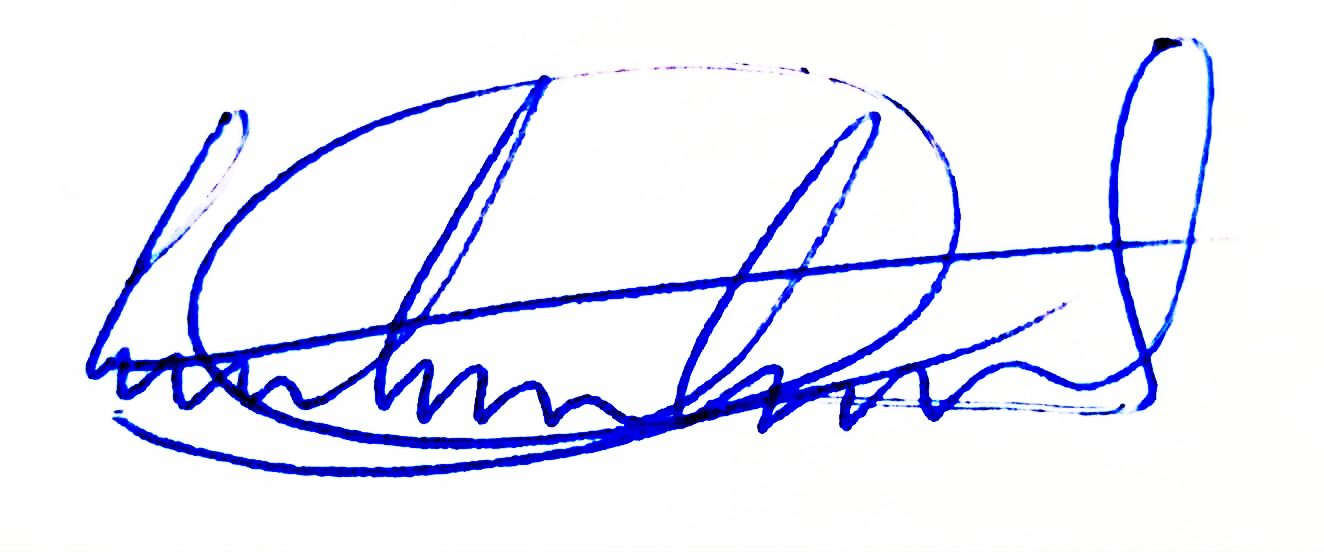
\includegraphics[height=1cm]{Figuras/firma_esau.jpg}
        
    \end{minipage}
    \hfill
    \begin{minipage}[t]{0.45\textwidth}
        \centering
        
        Dr. Ricardo Ramos Aguilar
        
        \vspace{1cm}

    \end{minipage}
    
\end{center}
\vspace{1cm}

\raggedleft{Tlaxcala, Tlaxcala, a \textbf{29} de \textbf{10} de \textbf{2025} }

\vspace{1cm}

\begin{center}
    \textcolor{guindaIPN}{\rule{12cm}{0.8mm}}\\
    \Large
    \textcolor{guindaIPN}{\textit{``La Técnica al Servicio de la Patria''}}
\end{center}
\justify
%------------------------------------------------------------

%------------------------------------------------------------
%    PREÁMBULO
%------------------------------------------------------------

\setcounter{page}{1}
\pagenumbering{roman}


\chapter*{Resumen}

En la actualidad, la generación de gemelos digitales de alta fidelidad mediante la reconstrucción tridimensional de interiores enfrenta desafíos significativos debido a la dependencia de sensores LiDAR de alto costo. Problemas como el ruido inherente a los sensores económicos, la pérdida de datos en superficies complejas y la elevada carga computacional han restringido el acceso a estas tecnologías para investigadores independientes y pequeñas empresas.

Con el fin de reducir esta brecha tecnológica, el presente documento expone el desarrollo de un \textit{pipeline} de reconstrucción 3D sustentado en visión artificial y una cámara de profundidad basada en el espectro infrarrojo activo (IR-D). El sistema integra modelos de aprendizaje profundo para el completado de profundidad y la segmentación semántica de instancias, lo que permite generar mallas tridimensionales coherentes a partir de la alineación óptica nativa del sensor.

El propósito es ofrecer representaciones digitales precisas para aplicaciones prácticas en diseño de interiores, realidad aumentada y robótica. La propuesta valida el uso de sensores infrarrojos accesibles (con un costo aproximado de entre \$2{,}000 y \$3{,}000 MXN), logrando una precisión geométrica competitiva expresada mediante un error cuadrático medio de alineación (ICP RMSE) de 2.52 cm y una integración volumétrica eficiente a través de la técnica TSDF.

\section*{Términos/Palabras Clave}

\begin{itemize}
    \item Visión artificial
    \item Aprendizaje profundo
    \item Reconstrucción 3D
    \item Imágenes infrarrojas (IR)
    \item Transferencia de dominio
\end{itemize}
%------------------------------------------------------------
% Índice General
\tableofcontents

\newpage
\renewcommand{\thepage}{\arabic{page}}
\setcounter{page}{1}
\pagestyle{fancy} 
\fancyhead[LE,RO]{\rightmark}
\fancyhead[RE,LO]{}


\chapter{Introducción}

La capacidad de manipular entornos digitales antes de que tomen una forma material ha revolucionado industrias como el diseño y la manufactura. Un ejemplo claro es la impresión 3D, que permite iterar y perfeccionar un objeto digitalmente antes de comprometer recursos físicos. La creación de un modelo digital previo al prototipo físico resulta, por tanto, altamente beneficiosa tanto en términos económicos como operativos.

Un ejemplo representativo se encuentra en la industria de la construcción con el concepto de ``orden de cambio'': un costo adicional que surge ante modificaciones imprevistas durante la obra. Estos costos pueden representar hasta un 10\% del presupuesto original, generando desperdicio de materiales y mano de obra. La modelación y el diseño en un entorno digital permiten anticipar este tipo de problemas, evitando sobrecostos y optimizando el uso de recursos desde las fases tempranas del proyecto.

Este mismo principio se aplica a la arquitectura y al diseño de interiores, donde la reconstrucción tridimensional de un espacio físico en un modelo digital constituye el primer paso fundamental. Específicamente, la capacidad de escanear y modelar espacios interiores comunes ---como habitaciones, oficinas o salas de estar--- permite una planificación y modificación sin restricciones, eliminando la necesidad de realizar costosos cambios físicos \cite{app15126681}.

Para que estas representaciones digitales sean útiles en aplicaciones prácticas ---como el diseño de interiores, la realidad aumentada o la robótica---, se requiere que la reconstrucción sea dimensionalmente coherente y de alta fidelidad visual. Es decir, el modelo debe capturar fielmente la escala y las proporciones del entorno real, garantizando una planificación espacial fiable y reproducible.

Alcanzar dicho nivel de fidelidad ha dependido históricamente de equipos de escaneo profesional como los escáneres LiDAR, cuyo alto costo limita considerablemente su accesibilidad. Esta situación ha motivado la búsqueda de métodos alternativos capaces de lograr reconstrucciones de alta calidad mediante el uso de sensores económicos.

En este trabajo se explora el potencial de las cámaras de profundidad basadas en luz estructurada e infrarrojo activo. Al integrar técnicas avanzadas de aprendizaje profundo con métodos de fusión volumétrica, se propone un sistema capaz de compensar las limitaciones físicas de estos sensores económicos, habilitando la creación de modelos 3D precisos y semánticamente segmentados sin necesidad de hardware de alta gama.

%------------------------------------------------------------

\section{Planteamiento del Problema}

La reconstrucción tridimensional de alta calidad es un área central en los campos de la visión artificial y los gráficos por computadora, principalmente porque permite crear gemelos digitales de entornos reales \cite{fuller2020digital}, los cuales sirven como base para aplicaciones como la realidad virtual, los videojuegos y los simuladores de entrenamiento \cite{technologies12030040,zhang2015real}. Esta tecnología tiene diversas utilidades prácticas; por ejemplo, facilita la modificación de obras arquitectónicas, dado que resulta más eficiente y económico manipular un entorno digital que uno físico: los cambios de diseño, materiales o distribución pueden ejecutarse de forma instantánea y reversible en un entorno de software, eliminando los costos de material y mano de obra que implicaría un prototipo físico.

Sin embargo, el proceso presenta desafíos técnicos considerables. Las reconstrucciones 3D realizadas con cámaras de bajo costo suelen ser ruidosas e incompletas, debido a que el sensor de profundidad infrarrojo falla al interactuar con determinadas superficies \cite{afzal2025improving}. Por ejemplo, los materiales brillantes o transparentes dispersan o transmiten la señal luminosa de forma errática, mientras que los objetos distantes devuelven un retorno demasiado débil para una medición precisa. A causa de estos fallos del sensor, obtener modelos tridimensionales de alta calidad sigue siendo un desafío abierto para los sistemas actuales \cite{6594910}.

Esto genera una clara barrera de accesibilidad. Por un lado, existen cámaras de profundidad asequibles como la serie Intel RealSense o la Azure Kinect; por el otro, se encuentran los escáneres LiDAR profesionales de marcas como Faro o Leica, que ofrecen precisión milimétrica. El problema radica en el desequilibrio entre ambas opciones: los equipos económicos presentan los fallos del sensor ya mencionados, mientras que los equipos de alta precisión tienen un costo prohibitivo para muchas aplicaciones e instituciones.

Además de las fallas en superficies reflectantes, los sistemas tradicionales que intentan sincronizar el canal de color (RGB) con el de profundidad (D) suelen presentar problemas de desalineación óptica, especialmente cuando las condiciones de iluminación ambiental varían. Por ello, operar exclusivamente en el espectro infrarrojo nativo del sensor constituye una alternativa más estable, aunque exige algoritmos avanzados capaces de interpretar la geometría de la escena sin depender del color visible.

Finalmente, para asegurar que la solución propuesta sea viable y cuantificable, la calidad de la reconstrucción se evaluará mediante métricas orientadas a la coherencia geométrica y la eficiencia de la odometría visual. La precisión del registro espacial se medirá a través del Error Cuadrático Medio de la alineación iterativa de puntos (ICP RMSE), el cual cuantifica la desviación local entre fotogramas consecutivos. Asimismo, la robustez de la trayectoria se validará mediante el parámetro de \textit{Fitness} del algoritmo ICP, que indica la fracción de correspondencias exitosas. Por último, la integridad y viabilidad del gemelo digital se evaluarán mediante métricas de complejidad de malla, analizando la reducción de polígonos y vértices tras la integración volumétrica (TSDF) y el filtrado espacial, con el objetivo de obtener un modelo ligero y libre de artefactos estructurales.

\section{Objetivos}

\subsection{Objetivo General}

Desarrollar un sistema de reconstrucción tridimensional de alta fidelidad para entornos interiores, optimizado para el espectro infrarrojo, empleando hardware de bajo costo y técnicas avanzadas de aprendizaje profundo.

\subsection{Objetivos Específicos}

\begin{itemize}
    \item Mejorar la calidad de los mapas de profundidad mediante una reducción medible del ruido y de las áreas faltantes, utilizando una arquitectura Efficient-UNet para el completado denso de profundidad.
    \item Estimar con precisión la \textbf{trayectoria local} de la cámara entre fotogramas consecutivos mediante un esquema híbrido que integre odometría visual y refinamiento geométrico con el algoritmo ICP punto-a-plano. Se aclara que la evaluación de la trayectoria global acumulada requeriría un \textit{ground truth} externo (estación total o sistema de captura de movimiento), lo cual se identifica como un posible trabajo futuro para fortalecer la validación metodológica del sistema.
    \item Reconstruir superficies tridimensionales coherentes mediante la fusión volumétrica (TSDF) de datos infrarrojos, integrando segmentación semántica basada en los modelos YOLO11x-seg y FastSAM.
    \item Evaluar el desempeño del sistema empleando métricas de error cuadrático medio (ICP RMSE), nivel de ajuste (\textit{Fitness}) y complejidad de malla, con el fin de validar la precisión del gemelo digital generado.
\end{itemize}

\section{Justificación}

La reconstrucción 3D tiene diversas aplicaciones en múltiples ámbitos: en el diseño de interiores, permite crear entornos digitales más fáciles de manipular en comparación con los entornos físicos; en la industria del entretenimiento, posibilita simular interacciones en escenarios de mayor diversidad y complejidad \cite{app15126681}.

No obstante, la adopción masiva de esta tecnología se ve frenada por una brecha tecnológica significativa. Por un lado, los escáneres LiDAR profesionales ofrecen alta fidelidad geométrica; por el otro, los sensores de bajo costo, si bien son accesibles, producen reconstrucciones con ruido, oclusión y deriva considerable \cite{afzal2025improving,6594910}. Este desequilibrio entre calidad y accesibilidad implica que optar por equipos de gama baja conlleva un riesgo inherente en la calidad de los resultados obtenidos.

Este proyecto busca abordar dicha problemática proponiendo una arquitectura de software que compense las deficiencias del hardware económico. Para lograrlo, no solo se emplea un modelo Encoder-Decoder basado en la arquitectura Efficient-UNet para estimar la profundidad densa y corregir el ruido del sensor infrarrojo, sino que también se integra un filtrado semántico avanzado. Mediante el uso de modelos de detección y segmentación como YOLO11x-seg y FastSAM, el sistema puede identificar los objetos de la escena, aislar el ruido dinámico y mejorar tanto la estimación de la trayectoria como la calidad de la fusión volumétrica.

En el contexto nacional, la disponibilidad de reconstrucciones 3D a bajo costo tendría un impacto directo en las pymes de los sectores de construcción y diseño en México, permitiéndoles adoptar tecnologías de digitalización sin la inversión prohibitiva en hardware especializado. A nivel institucional, este trabajo aportará una herramienta accesible y robusta a los laboratorios de visión artificial y robótica, fortaleciendo futuras líneas de investigación en el área.

\section{Hipótesis}

La integración de modelos de aprendizaje profundo para la reconstrucción de profundidad, en conjunto con un sistema de odometría visual, permite compensar las deficiencias ópticas y el ruido inherente a los sensores infrarrojos de bajo costo. Se espera que este enfoque permita generar reconstrucciones tridimensionales de entornos reales con un error cuadrático medio (RMSE) inferior a 2 cm, demostrando así la viabilidad de prescindir de equipos de alto costo para obtener representaciones geométricas de alta calidad.

\section{Aportación Científica y/o Tecnológica}

La aportación principal de este trabajo es la integración, implementación y evaluación experimental de un \textit{pipeline} de reconstrucción 3D que opera exclusivamente sobre el espectro infrarrojo de un sensor de bajo costo, combinando completado de profundidad neuronal, segmentación semántica y odometría visual en un flujo de trabajo cohesivo. Si bien cada componente individual existe en la literatura, su adaptación conjunta al dominio infrarrojo ---incluyendo la transferencia de dominio de YOLO mediante pseudo-etiquetas automáticas y la estandarización métrica del sensor--- representa una contribución de integración tecnológica reproducible. El sistema está diseñado para que otros investigadores puedan replicarlo como base para trabajos en reconstrucción 3D con hardware accesible.


\chapter{Marco Teórico}

Para el desarrollo de este proyecto se han integrado diversas técnicas de visión computacional y aprendizaje profundo, abarcando desde el tratamiento de señales infrarrojas hasta la generación de mallas tridimensionales \cite{li2022high,tychola20223d}.

\section{Base de Datos y Adaptación de Dominio}

El sistema utiliza el conjunto de datos \textbf{SUN RGB-D} para el entrenamiento y la validación \cite{song2015sun}. Esta base de datos contiene más de 10{,}000 imágenes de interiores que permiten al modelo aprender la relación entre la apariencia visual de una escena y su estructura geométrica en profundidad.

Sin embargo, dado que la cámara RealSense D430 captura imágenes en el espectro infrarrojo para evitar errores de paralaje, se aplicó una técnica de \textbf{transferencia de dominio} (\textit{domain transfer}). El modelo, inicialmente entrenado con datos RGB, fue ajustado mediante un proceso de \textit{fine-tuning} sobre un conjunto de datos propio de 319 fotogramas infrarrojos. Es importante reconocer que este conjunto de imágenes es reducido para un problema de generalización visual; en consecuencia, la capacidad del modelo para operar correctamente en escenas de interiores con características distintas a las capturadas no está completamente demostrada y representa una limitación explícita del trabajo.


\section{Preprocesamiento y Filtrado Espacial}

Con el fin de maximizar la calidad de los datos previo a la reconstrucción, se implementó una etapa de preprocesamiento que depura la señal del sensor:

\begin{itemize}
    \item \textbf{Filtro Bilateral:} A diferencia de los filtros de suavizado convencionales, el filtro bilateral preserva los bordes nítidos de los objetos al ponderar la diferencia de intensidad entre píxeles adyacentes \cite{paris2022survey}. Esta propiedad es fundamental para evitar que las aristas del mobiliario se distorsionen durante el proceso de reconstrucción.
    \item \textbf{Z-cropping (Recorte de Profundidad):} Con el fin de optimizar la carga computacional y concentrar la reconstrucción en el mobiliario de interés, se aplica un filtro de umbral en el eje Z (típicamente entre 0.3 m y 2.8 m). Esto permite eliminar automáticamente el techo y el suelo de la escena, reduciendo el ruido estructural del entorno.
    \item \textbf{Normalización de 16 bits:} Los mapas de profundidad crudos se capturan en formato de 16 bits (milímetros). El sistema convierte estos valores a metros utilizando precisión de punto flotante para su procesamiento correcto en las redes neuronales.
\end{itemize}

\subsection{Arquitecturas de Aprendizaje Profundo}

El \textit{pipeline} emplea dos modelos especializados para comprender y completar la información de la escena:

\subsubsection{Efficient-UNet para Completado de Profundidad}

Se utiliza una arquitectura basada en \textbf{EfficientNet-B0} como codificador (\textit{encoder}). La selección de esta arquitectura está respaldada por los resultados reportados en el trabajo original de \cite{tan2019efficientnet}, que demuestra que EfficientNet-B0 logra mayor precisión que ResNet-50 en ImageNet (77.1\% vs.\ 76.0\%) utilizando 4.8 veces menos parámetros (5.3M vs.\ 25.6M) y 10.5 veces menos operaciones de punto flotante (0.39B vs.\ 4.1B FLOPS). Esta eficiencia computacional es relevante para el contexto del proyecto, donde el codificador debe operar dentro de un \textit{pipeline} que también ejecuta segmentación semántica en la misma GPU. El modelo procesa tensores de 5 canales (IR, profundidad y máscara) para predecir un mapa de profundidad denso, rellenando los vacíos generados por el sensor.

\subsubsection{YOLO11x-seg y Segmentación Semántica}

Para lograr una comprensión integral de la escena, se integra el modelo \textbf{YOLO11x-seg}, que permite la detección y segmentación de instancias en tiempo real. En combinación con \textbf{FastSAM}, este módulo identifica objetos específicos (sillas, mesas, estantes, entre otros), permitiendo al sistema ignorar los elementos dinámicos o irrelevantes durante la etapa de fusión 3D.


\section{Reconstrucción y Fusión Volumétrica}

El paso final consiste en transformar la secuencia de imágenes procesadas en un modelo tridimensional sólido:

\begin{itemize}
    \item \textbf{Odometría Visual (ICP Point-to-Plane):} Para determinar la posición de la cámara a lo largo de la secuencia, se emplea el algoritmo de \textbf{Punto Cercano Iterativo} (\textit{Iterative Closest Point}). La variante \textit{point-to-plane} resulta más robusta en entornos de interiores, ya que utiliza las normales de las superficies para lograr una alineación más precisa entre fotogramas sucesivos. Esta variante, propuesta por \cite{rusinkiewicz2001efficient}, minimiza la distancia punto-a-plano en lugar de punto-a-punto, ofreciendo una convergencia más rápida en superficies planas como paredes y mobiliario.
    \item \textbf{Fusión TSDF (\textit{Truncated Signed Distance Function}):} En lugar de acumular puntos de manera independiente, el sistema utiliza una cuadrícula volumétrica de vóxeles con una resolución de 8 mm. Cada vóxel almacena la distancia firmada a la superficie más cercana, lo que permite promediar el ruido a lo largo del tiempo y generar mallas continuas y cerradas geométricamente.
    \item \textbf{Post-procesamiento de Malla:} Una vez generada la malla, se aplica el filtro de \textbf{Taubin} para suavizar la superficie sin reducir el volumen de los objetos, seguido de una decimación de triángulos para obtener un modelo ligero y exportable de aproximadamente 300{,}000 polígonos\footnote{G. Taubin, ``A Signal Processing Approach to Fair Surface Design,'' \textit{Proceedings of the 22nd Annual Conference on Computer Graphics and Interactive Techniques} (SIGGRAPH), 1995.}.
\end{itemize}

\section{Métricas de Evaluación de Modelos de Aprendizaje Profundo}

Se utilizan métricas específicas para evaluar la precisión de los modelos de aprendizaje profundo, asegurando que cada componente del sistema opere de manera óptima antes de la etapa de reconstrucción.

\textbf{Para el modelo de completado de profundidad (Efficient-UNet):}
\begin{itemize}
    \item \textbf{Edge-Aware Loss (Función de Pérdida):} Esta función personalizada, diseñada para el entrenamiento del modelo de profundidad, combina el Error Absoluto Medio (MAE o L1 Loss) con una penalización basada en diferencias finitas (gradientes espaciales). Su propósito es obligar a la red neuronal a preservar la nitidez de los bordes de los objetos, evitando que el modelo genere transiciones difusas en zonas que físicamente presentan discontinuidades abruptas de profundidad.
    \item \textbf{Precisión Delta ($\delta < 1.25$):} Es la métrica estándar para la evaluación de la estimación de profundidad monocular. Calcula el porcentaje de píxeles predichos cuyo error relativo es inferior al 25\% respecto a la distancia real medida por el sensor, excluyendo los píxeles vacíos mediante la aplicación de máscaras de validez.
\end{itemize}


\textbf{Para el modelo de segmentación de instancias (YOLO11x-seg):}
\begin{itemize}
    \item \textbf{Precisión Media Promedio (mAP --- \textit{Mean Average Precision}):} Es la métrica principal empleada en la literatura para evaluar tareas de detección y segmentación. Se basa en el cálculo de la Intersección sobre Unión (IoU), midiendo el grado de superposición entre la máscara de píxeles generada por el algoritmo y la silueta real del objeto en la escena. Un valor de mAP elevado garantiza que el filtro semántico excluirá únicamente las regiones correctas, sin eliminar partes estructuralmente relevantes de la escena.
\end{itemize}

\section{Métricas de Evaluación de la Reconstrucción}

Para validar la precisión del sistema y la calidad de la reconstrucción generada, se emplean métricas que permiten cuantificar el error de alineación y la eficiencia del modelo final:

\begin{itemize}
    \item \textbf{Error Cuadrático Medio (RMSE):} En el contexto del algoritmo ICP, el RMSE (\textit{Root Mean Square Error}) mide la distancia promedio entre los puntos de dos nubes una vez alineadas. Un valor bajo indica que las superficies coinciden de forma casi exacta, lo cual es esencial para una reconstrucción fiel a la geometría real.
    \item \textbf{Fitness (Nivel de Ajuste):} Esta métrica indica el porcentaje de puntos que el algoritmo logró emparejar exitosamente entre dos fotogramas consecutivos. Un valor de \textit{Fitness} cercano al 100\% significa que la cámara mantuvo un rastreo robusto de la escena, evitando que el modelo tridimensional presente discontinuidades o desalineaciones acumuladas.
    \item \textbf{Densidad y Complejidad de Malla:} Se evalúa el número de vértices y triángulos que componen la malla final. El objetivo es alcanzar un equilibrio adecuado: contar con suficientes polígonos para representar los detalles del mobiliario y la arquitectura interior, pero reducirlos al mínimo necesario para que el modelo sea ligero y manejable en cualquier software de diseño.
\end{itemize}

\newpage 

\chapter{Estado del Arte}

La reconstrucción tridimensional de escenas interiores a partir de sensores de profundidad constituye un campo de investigación activo y diverso dentro de la visión por computadora. Históricamente dominado por el uso de cámaras RGB-D, este campo ha evolucionado para abordar los desafíos clave del proceso, que abarcan desde la adquisición y el procesamiento de datos ruidosos hasta la estimación precisa de la pose de la cámara y la fusión coherente de múltiples vistas para generar un modelo tridimensional final.

El objetivo primordial es superar las limitaciones inherentes de los sensores de bajo costo, como el ruido en los mapas de profundidad y la incapacidad para medir con precisión superficies reflectantes o transparentes \cite{afzal2025improving}. Dicho ruido se manifiesta como huecos o datos faltantes, un problema recurrente cuando el sensor infrarrojo de la cámara interactúa con materiales brillantes, translúcidos o superficies situadas a gran distancia.

La estimación precisa de la pose de la cámara es un pilar fundamental de todo el proceso, ya que pequeños errores de seguimiento pueden acumularse a lo largo de la secuencia y provocar un efecto conocido como \textit{drift}, el cual se traduce en desalineaciones, paredes duplicadas e inconsistencias geométricas en el modelo final.

Para resolver estos problemas, el campo ha evolucionado desde enfoques algorítmicos clásicos hacia la integración progresiva de técnicas de aprendizaje profundo (\textit{deep learning}). Estos modelos modernos son capaces de inferir información geométrica a partir de señales visuales —ya sea en el espectro de color visible o mediante visión infrarroja—, lo que permite rellenar los vacíos dejados por el sensor de profundidad y mejorar la robustez general del sistema.

El flujo de trabajo para la reconstrucción tridimensional de alta calidad generalmente comprende las siguientes etapas:
\begin{itemize}
    \item \textbf{Procesamiento y relleno de datos de profundidad:} Mejorar la calidad de los mapas de profundidad eliminando el ruido y rellenando las áreas faltantes mediante técnicas algorítmicas o basadas en aprendizaje profundo.
    \item \textbf{Comprensión y segmentación semántica:} Analizar los fotogramas para identificar los objetos presentes en la escena y aislar los elementos dinámicos que puedan corromper el modelo espacial.
    \item \textbf{Estimación de la pose de la cámara (Odometría):} Determinar con precisión la posición y orientación de la cámara en cada fotograma para alinear correctamente las diferentes vistas.
    \item \textbf{Fusión volumétrica y reconstrucción de superficies:} Integrar los datos de profundidad alineados de múltiples vistas en un único modelo tridimensional coherente.
\end{itemize}

\section{Análisis de Trabajos Relacionados}

El relleno de profundidad en imágenes RGB-D es una etapa esencial para el proyecto, especialmente cuando el objetivo es realizar la reconstrucción de forma rentable y accesible. Para abordar este problema, el estudio \textit{Deep Depth Densification} \cite{chen2018estimating} propone una arquitectura de codificador-decodificador basada en DenseNet de múltiples escalas. Durante el entrenamiento, los mapas de profundidad dispersos (S1 y S2) se inyectan a múltiples escalas para preservar la información de profundidad a lo largo de toda la red, la cual predice un mapa de profundidad residual que se suma a S1 para generar la salida densa final. Los resultados obtenidos son comparables a los de los sensores de profundidad de consumo (error aproximado del 1\% con una escala de 16$\times$16), lo que lo convierte en una referencia metodológica relevante para este trabajo.

El siguiente paso, una vez estimada la profundidad, es la estimación de la pose de la cámara, indispensable para una reconstrucción precisa. En este sentido, el estudio de \cite{tang2021learning} propone \textit{Dense Scene Matching} (DSM), un método independiente de la escena para la estimación de la pose a partir de imágenes RGB. A diferencia de los enfoques tradicionales específicos por escena, DSM construye un volumen de costos entre una imagen de consulta y una escena 3D de referencia para predecir mapas de coordenadas densos, lo que le permite generalizarse a escenas arbitrarias sin necesidad de reentrenamiento. Este método logra precisión de vanguardia en entornos interiores (conjunto de datos 7-Scenes), superando a SANet (\textit{Scene Agnostic Network}) \cite{9009066} entre un 1.6\% y un 16\% en precisión a lo largo de todas las secuencias evaluadas.

En cuanto a la etapa de reconstrucción propiamente dicha, el estudio de \cite{li2022high} ofrece una revisión comparativa de los métodos existentes. En la estimación de la pose de la cámara se analizan métodos basados en ICP (\textit{Iterative Closest Point}), en características visuales y métodos híbridos. Para la reconstrucción de superficies, se revisan técnicas de fusión volumétrica, optimización y finalización de mallas. Empleando \textit{benchmarks} como ICL-NUIM y TUM RGB-D, el estudio demuestra que \textit{BundleFusion} \cite{10.1145/3072959.3054739} y \textit{UncertaintyAware} \cite{tan2025uncertaintyawarenormalguidedgaussiansplatting} obtienen el mejor rendimiento en precisión de seguimiento y reconstrucción de superficies.

Otro trabajo relevante \cite{li2018elaborate} emplea cámaras de profundidad de consumo como la Kinect. En dicho sistema, la escena se divide en segmentos lógicos según su contenido (objetos individuales, paredes, etc.) en lugar de un número fijo de fotogramas, lo que mejora la precisión de la alineación. Estos segmentos se unen mediante una combinación de ajuste fino local con ICP, superando las técnicas existentes en precisión y manejando eficientemente los desafíos propios de los entornos reales, lo que lo hace especialmente pertinente para aplicaciones de robótica y realidad virtual.

%------------------------------------------------------------
\newpage

\begin{longtblr}[
  caption = {Estudios Relacionados (Parte 2: Reconstrucción de Escenas Interiores)},
  label = {tab:estudios_2},
]{
  colspec = {|X|X|X|X|X|},
  rowhead = 1,
  hlines,
  row{even} = {},
  row{1} = {bg=vinoclaro, fg=white, font=\bfseries},
} 
Título & Metodología & Conjunto de datos & Resultados & Limitaciones\\

High-quality indoor scene 3D reconstruction with RGB-D cameras: A brief review &
Revisión de métodos de procesamiento de profundidad, estimación de poses (ICP, características, híbridos) y reconstrucción de superficies (fusión, optimización, finalización). &
Múltiples conjuntos de datos: TUM RGB-D, ICL-NUIM, ScanNet, Matterport3D, Replica, etc. Evaluación con \textbf{ATE} (Error Absoluto de Trayectoria) y \textbf{RMSE} (Error Cuadrático Medio). &
BundleFusion: ATE RMSE $\sim$15 mm; UncertaintyAware: mejor precisión en superficies (error mediano $\sim$4--6 mm). InfiniTAM v3: mayor velocidad (910 fps en GPU). &
Limitado a entornos interiores. Calidad afectada por superficies reflectantes o transparentes. Dependencia de hardware e iluminación. Los métodos de \textit{deep learning} requieren grandes conjuntos de datos de entrenamiento.
\\

FusionVision: A Comprehensive Approach of 3D Object Reconstruction
&
Pipeline que combina \textbf{YOLO} (\textit{You Only Look Once}) para detección 2D, \textbf{FastSAM} (\textit{Fast Segment Anything Model}) para segmentación y alineación RGB-D para reconstrucción 3D. &
Conjunto de datos propio de 100 imágenes (vaso, botella, etc.) capturadas con Intel RealSense D435i. &
YOLO: mAP50 97.92\%. FastSAM: IoU 0.94. Tasa de fotogramas: 27.3 fps en GPU RTX 2080 Ti. Eliminación del 85\% del ruido. &
Limitado a objetos pequeños y escenas interiores simples. Dependiente de la calibración RGB-D. Requiere GPU para operación en tiempo real. No evalúa oclusión severa.
\\

\end{longtblr}

\begin{longtblr}[
  caption = {Estudios Relacionados (Parte 3: SLAM y Componentes de Reconstrucción)},
  label = {tab:estudios_3},
]{
  colspec = {|X|X|X|X|X|},
  rowhead = 1,
  hlines,
  row{even} = {},
  row{1} = {bg=vinoclaro, fg=white, font=\bfseries},
} 
Título & Metodología & Conjunto de datos & Resultados & Limitaciones\\

Learning Camera Localization via Dense Scene Matching
&
Método de localización agnóstico a la escena (DSM) mediante un volumen de costo entre la imagen de consulta y escenas de referencia. Esquema \textit{coarse-to-fine} con \textbf{PnP} (\textit{Perspective-n-Point}) + \textbf{RANSAC} (\textit{Random Sample Consensus}).
&
Entrenado en ScanNet. Evaluado en 7-Scenes (interior) y Cambridge Landmarks (exterior). Utiliza ResNet50-FPN.
&
Precisión en 7-Scenes: 0.68--1.33° (rotación), 0.01--0.05 m (traslación). Supera a SANet. Velocidad: 0.21 s por fotograma.
&
Requiere imágenes de referencia con coordenadas 3D. Sensible a la calidad de la recuperación de imágenes. No opera en escenas sin solapamiento visual con la base de datos.
\\
Uncertainty-Aware Normal-Guided Gaussian Splatting
&
UNG-GS: Framework basado en 3D Gaussian Splatting con un campo de incertidumbre espacial (\textbf{SUF}) explícito. Incluye renderizado de profundidad y normales.
&
DTU, Tanks \& Temples (TnT), Mip-NeRF 360.
&
Mejora la distancia de Chamfer (CD) en DTU (0.62 mm) y el F1-score en TnT (0.39). Supera a 2DGS, GOF, RaDe-GS y PGSR.
&
Dificultades con superficies reflectantes o transparentes. Dependencia de COLMAP para la nube de puntos inicial.
\\
A Survey of Visual SLAM Methods
&
Revisión de métodos de V-SLAM (\textit{Visual SLAM}), clasificados por tipo de sensor (monocular, estéreo, RGB-D) y enfoque algorítmico (directo, basado en características, semántico).
&
KITTI, EuRoC, TUM-RGBD, ICL-NUIM, ETH3D, TartanAir, InteriorNet, entre otros.
&
Análisis comparativo de métodos, métricas (ATE, RPE), tendencias actuales, desafíos abiertos y direcciones futuras de investigación.
&
No propone un método nuevo. Su alcance se limita a la revisión y comparativa de trabajos existentes. No incluye experimentos propios.
\\
\end{longtblr}


\newpage

El análisis de los trabajos presentados en las tablas del estado del arte revela una clara tendencia hacia el uso de redes neuronales profundas como principal herramienta para abordar los desafíos de la reconstrucción 3D. Sin embargo, las arquitecturas y enfoques específicos varían significativamente según la naturaleza del problema. A continuación, se describen los grupos de metodologías más relevantes identificados en la literatura.

\textbf{Arquitecturas Neuronales para la Interpretación Geométrica:} Una parte considerable de los estudios emplea arquitecturas de redes neuronales especializadas para procesar datos geométricos. Por ejemplo, se observan modelos que combinan Redes Neuronales Convolucionales (CNN) con Transformers para reconstruir secuencias de operaciones en modelos CAD \cite{app15126681}, aprovechando la capacidad de las CNN para extraer características locales y la de los Transformers para modelar dependencias secuenciales a largo plazo.

\textbf{\textit{Pipelines} Basados en Comprensión Semántica de la Escena:} Un enfoque cada vez más extendido consiste en no tratar la reconstrucción como un problema puramente geométrico, sino en incorporarle una capa de comprensión semántica. El sistema FusionVision \cite{el2024fusionvision} es un claro ejemplo de esta tendencia, al proponer un \textit{pipeline} que primero detecta objetos en 2D mediante YOLO y posteriormente los segmenta con FastSAM. Al identificar y delimitar los elementos de la escena, la reconstrucción 3D resultante es más precisa y semánticamente estructurada, lo cual resulta fundamental para aplicaciones de robótica o realidad aumentada donde la interacción con objetos específicos es requerida.

\section{Conclusión del Análisis de la Literatura}

A lo largo del análisis de la literatura y el estado del arte se ha podido constatar una constante evolución en los métodos de reconstrucción tridimensional. Esta evolución se debe principalmente a la incorporación de nuevas tecnologías, que han propiciado la transición desde algoritmos clásicos hacia métodos basados en aprendizaje automático. Estos últimos han demostrado ser una alternativa viable para sensores de bajo costo, sin la necesidad de recurrir a equipos de alta gama, al abordar eficazmente los problemas de ruido en los mapas de profundidad y la pérdida de datos, particularmente en superficies irregulares \cite{afzal2025improving}.

Para llevar a cabo un análisis crítico de la literatura, resultó necesario separar el problema en las tres etapas identificadas: (1) el preprocesamiento y relleno de datos de profundidad, (2) la estimación de la posición de la cámara y (3) la fusión de vistas para el modelado de la superficie.

Dicho análisis revela limitaciones clave que motivan la propuesta de este proyecto. En la estimación de pose, si bien \textit{Dense Scene Matching} (DSM) \cite{tang2021learning} es un método potente, su principal limitación (identificada en la Tabla \ref{tab:estudios_3}) radica en su dependencia de una base de datos de escenas de referencia con coordenadas 3D conocidas, lo que lo hace poco práctico para la reconstrucción en tiempo real de entornos desconocidos. Por su parte, sistemas integrales de alta precisión como \textit{BundleFusion} \cite{10.1145/3072959.3054739} —mencionado en \cite{li2022high}— son reconocidos por su elevada carga computacional, lo que limita su viabilidad en entornos con recursos restringidos.

La principal brecha (\textit{gap}) identificada es la ausencia de un \textit{pipeline} que integre de forma eficiente un relleno de profundidad robusto con una estimación de pose que sea precisa pero computacionalmente accesible. Concretamente: \textit{Deep Depth Densification} \cite{chen2018estimating} resuelve el relleno pero no contempla segmentación semántica para filtrar elementos dinámicos, lo que vuelve su odometría vulnerable a ruido en escenas con personas u objetos en movimiento. DSM \cite{tang2021learning} aborda la localización, pero requiere una base de datos de referencia preconstruida con coordenadas 3D, lo que lo hace inviable para reconstruir entornos nuevos en tiempo real. \textit{BundleFusion} \cite{10.1145/3072959.3054739} logra alta precisión, pero su carga computacional impide su uso en hardware de consumo. FusionVision \cite{el2024fusionvision} introduce la segmentación semántica en el \textit{pipeline}, pero fue diseñado y validado únicamente para objetos pequeños y aislados, sin escenas de interiores completas ni oclusión severa.

Por lo tanto, este proyecto toma a \textbf{FusionVision} \cite{el2024fusionvision} como punto de partida metodológico e incorpora dos modificaciones concretas para escalar su alcance: (1) agrega un módulo de completado de profundidad previo (inspirado en \cite{chen2018estimating}) que entrega mapas densos al algoritmo de odometría, reduciendo los fallos de rastreo causados por huecos en el sensor, y (2) reemplaza la alineación RGB-D de FusionVision por odometría ICP punto-a-plano sobre datos exclusivamente infrarrojos, eliminando los errores de paralaje que afectan a los sistemas con cámara de color. La contribución del trabajo reside en esta integración sobre el espectro infrarrojo y en su validación experimental sobre secuencias continuas de escenas interiores completas.

\chapter{Metodología}

La metodología empleada en este proyecto sigue una secuencia lógica de pasos, resumida visualmente en el diagrama de flujo presentado en la Figura \ref{fig:flow-chart}.

Es importante señalar que, si bien el \textit{pipeline} está diseñado para ejecutarse de forma secuencial, cada componente principal fue desarrollado y evaluado de manera individual antes de su integración. Los resultados reportados en el capítulo siguiente reflejan el desempeño de cada módulo por separado (completado de profundidad, segmentación semántica) y el desempeño del sistema integrado sobre una secuencia real de 338 fotogramas capturados, de los cuales 319 fueron integrados exitosamente tras el filtrado por ICP. Esta distinción es relevante para interpretar correctamente el alcance experimental del trabajo.

El proceso comienza con la \textbf{adquisición de datos} mediante una cámara de profundidad Intel RealSense D430. A diferencia de los métodos tradicionales, el sistema captura imágenes en el espectro infrarrojo nativo junto con sus mapas de profundidad correspondientes, asegurando una alineación óptica perfecta desde el momento de la grabación.

Tras esta captura, la información cruda ingresa en una etapa crítica de \textbf{procesamiento}, en la cual el sistema realiza el trabajo computacional más intensivo: un modelo de aprendizaje profundo rellena los vacíos generados por el ruido del sensor y, de manera simultánea, un filtro semántico identifica los objetos presentes en la escena, descartando los elementos dinámicos que podrían comprometer la integridad del modelo.

Una vez que los mapas de profundidad han sido densificados y depurados, el núcleo del sistema procede a la \textbf{reconstrucción geométrica}. En esta etapa se calcula la trayectoria exacta seguida por la cámara a través del espacio, se alinean las superficies de manera incremental y se construye una malla tridimensional sólida mediante la integración de todas las vistas.

Finalmente, el modelo 3D resultante es sometido a una fase de optimización para reducir el número de polígonos y obtener un archivo de tamaño manejable, seguida de una evaluación matemática. La validación de la precisión geométrica mediante métricas de alineación interna permite comprobar la fidelidad del gemelo digital generado.

\begin{figure}[htbp]
    \centering
    \makebox[\linewidth][c]{%
        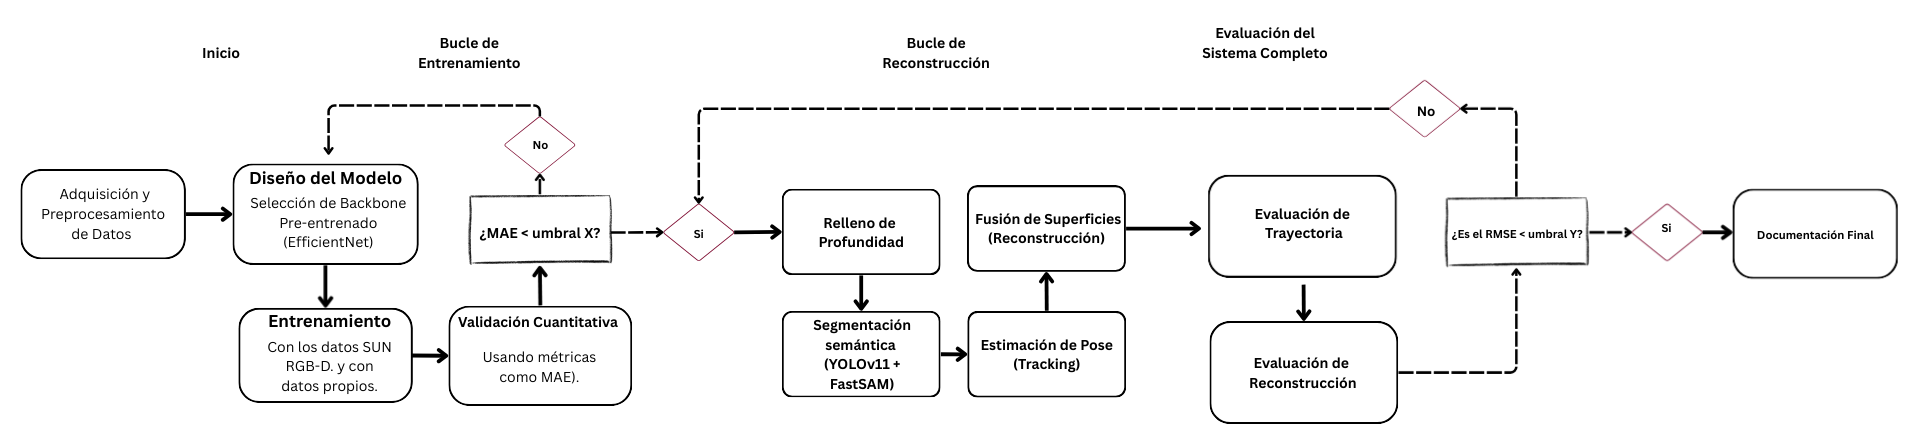
\includegraphics[width=1.25\linewidth]{Figuras/methodology_flow_chart.png} 
    }
    \caption{Diagrama de proceso de la metodología propuesta.}
    \label{fig:flow-chart}
\end{figure}


\section{Entorno de Desarrollo}

El proyecto se desarrolla utilizando el siguiente hardware y software:

\begin{itemize}
    \item \textbf{Hardware de Cómputo:} GPU NVIDIA RTX 3080 Ti, empleada para acelerar la inferencia de los modelos de aprendizaje profundo. Su uso resulta indispensable dado el alto costo computacional de ejecutar simultáneamente la red de completado de profundidad y los modelos de segmentación semántica durante el bucle de reconstrucción.
    \item \textbf{Lenguaje de Programación:} Python 3.12.
    \item \textbf{Framework de Deep Learning:} PyTorch. A diferencia de alternativas como TensorFlow, PyTorch fue seleccionado por su flexibilidad en el manejo dinámico de tensores, característica fundamental tanto para construir la arquitectura Encoder-Decoder como para implementar la función de pérdida personalizada \textit{EdgeAwareLoss}.
    \item \textbf{Procesamiento 3D:} Librería Open3D, empleada para la manipulación de nubes de puntos, la implementación del algoritmo ICP y la fusión volumétrica TSDF.
    \item \textbf{Utilidades:} OpenCV para el preprocesamiento de imágenes (filtrado bilateral, entre otros) y NumPy para operaciones matriciales de alto rendimiento.
\end{itemize} 

\section{Arquitectura del Sistema Propuesto}

El sistema opera como un \textit{pipeline} modular y secuencial, diseñado para integrar etapas que en la literatura se abordan de manera independiente. Esta arquitectura híbrida unifica tres bloques principales orientados a resolver las limitaciones físicas de los sensores de bajo costo:

\begin{itemize}
    \item \textbf{Preprocesamiento Inteligente:} Se adaptó una arquitectura de red neuronal (Efficient-UNet) para recibir un tensor de 5 canales (IR, profundidad y máscara), con el objetivo de reparar la geometría incompleta del sensor infrarrojo y rellenar los vacíos de profundidad generados por el ruido óptico.
    \item \textbf{Filtrado Semántico:} Se incorporan modelos de detección y segmentación (YOLO11x-seg y FastSAM) para comprender la composición de la escena e identificar el mobiliario, permitiendo al sistema discriminar y suprimir los elementos dinámicos que puedan introducir ruido en el mapa espacial.
    \item \textbf{Fusión Geométrica:} Se emplean algoritmos de odometría visual (ICP punto-a-plano) y reconstrucción volumétrica (TSDF) para alinear espacialmente todos los fotogramas procesados y consolidarlos en una malla tridimensional coherente.
\end{itemize}

\section{Adquisición de Datos y Adaptación de Dominio}

Para que las redes neuronales operen correctamente, es necesario que aprendan a partir de ejemplos representativos. El entrenamiento del modelo de completado de profundidad se estructuró en dos fases complementarias:

\textbf{1. Preentrenamiento con SUN RGB-D:}
En una primera etapa, el modelo aprendió la relación entre apariencia visual y profundidad geométrica utilizando el conjunto de datos SUN RGB-D \cite{song2015sun}. De este conjunto se utilizaron \textbf{7{,}245 imágenes para entrenamiento} y \textbf{319 imágenes para validación} (con 5{,}449 instancias anotadas distribuidas en 17 clases). Esta base de datos fue seleccionada por su diversidad de escenas de interiores y por incluir etiquetas de segmentación semántica. La Figura \ref{fig:sun_RGBD} muestra un ejemplo representativo.

\begin{figure}[H]
    \centering
    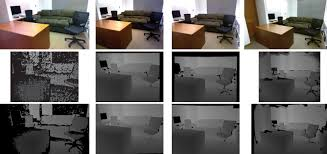
\includegraphics[width=0.8\linewidth]{Figuras/SUN-RGB.jpeg}
    \caption{Ejemplo de la base de datos SUN RGB-D. \cite{SUN-RGBD-DATASET-PAPER}}
    \label{fig:sun_RGBD}
\end{figure}

\textbf{2. Captura Propia y Transferencia al Infrarrojo:}

Dado que el objetivo del proyecto es operar con hardware de bajo costo, se evaluaron diversas alternativas de sensores de profundidad. La Tabla \ref{tab:comparativa_camaras} presenta las opciones consideradas. Finalmente, se seleccionó la cámara \textbf{Intel RealSense D430}. Al constatar que los sistemas tradicionales presentan desalineación entre la lente de color y la de profundidad, se tomó la decisión de diseño de que el sistema operara exclusivamente en el espectro infrarrojo (IR) del sensor.

Para que el modelo preentrenado en RGB pudiera operar con imágenes en escala de grises, se capturó un conjunto de datos propio de \textbf{319 fotogramas infrarrojos} y se realizó un ajuste fino (\textit{fine-tuning}). Cabe señalar que este tamaño de conjunto es reducido para un problema de transferencia de dominio; en consecuencia, no se puede garantizar que el modelo generalice correctamente a entornos con condiciones de iluminación infrarroja o distribución espacial significativamente distintas de las del conjunto propio.

\begin{table}[H]
\centering
\caption{Comparativa de Cámaras de Profundidad Accesibles}
\label{tab:comparativa_camaras}
\begin{tabular}{l l p{7cm}}
\toprule
\textbf{Nombre} & \textbf{Precio (Aprox.)} & \textbf{Ventajas Principales} \\
\midrule
\textbf{Intel RealSense D430 / D435} & \$200 -- \$300 USD & 
\begin{itemize}[noitemsep, nolistsep, leftmargin=*]
    \item \textbf{Alineación Nativa:} Sensor infrarrojo activo estéreo de alta calidad, ideal para evitar errores de paralaje RGB.
    \item \textbf{Soporte:} SDK robusto (\texttt{librealsense}) con integración directa en Python.
\end{itemize} \\
\addlinespace
Microsoft Kinect v2 & \$30 -- \$60 USD (Usada) & 
\begin{itemize}[noitemsep, nolistsep, leftmargin=*]
    \item \textbf{Costo:} Opción más económica disponible en mercado de segunda mano.
    \item \textbf{Desventaja:} Hardware descontinuado, de tamaño considerable y con configuración compleja en sistemas Linux.
\end{itemize} \\
\addlinespace
Orbbec Gemini 335 & \$200 -- \$230 USD & 
\begin{itemize}[noitemsep, nolistsep, leftmargin=*]
    \item \textbf{Tecnología:} Active Stereo IR con IMU integrada.
    \item \textbf{Soporte:} Diseñada para robótica con SDK compatible con ROS 2.
\end{itemize} \\
\bottomrule
\end{tabular}
\end{table}

\begin{figure}[H]
    \centering
    \begin{subfigure}[b]{0.48\linewidth}
        \centering
        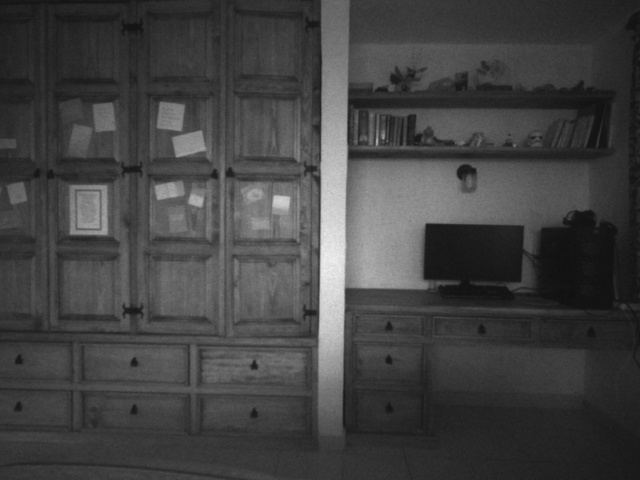
\includegraphics[width=\linewidth]{Figuras/yolo_data_0000.jpg}
        \caption{Imagen infrarroja (IR) de la secuencia de captura}
        \label{fig:ir_sample}
    \end{subfigure}
    \hfill
    \begin{subfigure}[b]{0.48\linewidth}
        \centering
        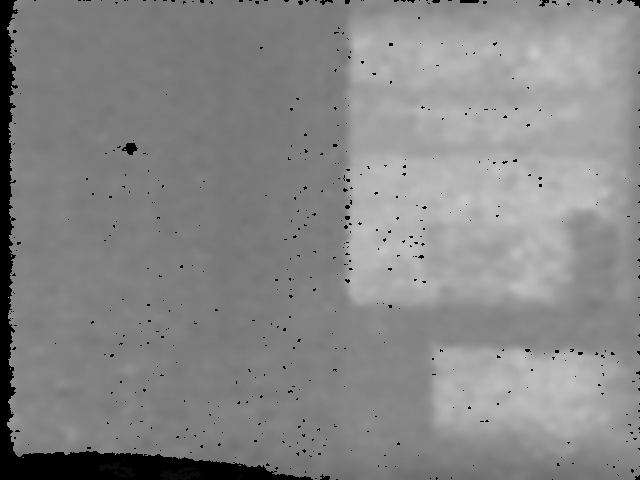
\includegraphics[width=\linewidth]{Figuras/yolo_data_Depth.png}
        \caption{Mapa de profundidad (Depth) correspondiente}
        \label{fig:depth_sample}
    \end{subfigure}
    \caption{Ejemplo de un par IR-Depth de la secuencia de 338 fotogramas capturada con la cámara RealSense D430. La imagen infrarroja (izquierda) muestra la escena en escala de grises, mientras que el mapa de profundidad (derecha) codifica la distancia en milímetros (formato Z16).}
    \label{fig:ir_depth_sample}
\end{figure}

\section{Preparación y Estandarización de Datos}

Para que las redes neuronales operen de manera predecible y estable, los datos de entrada no pueden introducirse en su formato crudo ni en resoluciones arbitrarias. Fue necesario establecer un protocolo estricto de estandarización tanto para la base de datos de entrenamiento (SUN RGB-D) como para el conjunto de datos capturado con hardware propio.

\subsection{Redimensionamiento y Verificación de Formatos}

Tanto las imágenes visuales como los mapas de profundidad se redimensionaron a una resolución estándar de \textbf{480$\times$640 píxeles}. Esta resolución fue seleccionada porque coincide con la relación de aspecto nativa del sensor infrarrojo (4:3) y representa un equilibrio óptimo: es suficientemente grande para conservar los detalles estructurales del mobiliario, pero lo bastante reducida para que el modelo Efficient-UNet pueda procesarla en la GPU sin saturar la memoria VRAM.

Adicionalmente, se implementó un paso crítico de verificación de dimensiones (canales). La primera capa de la red fue diseñada para recibir exactamente 5 canales. Dado que el sistema opera con una cámara monocromática (infrarroja), se adaptó la imagen IR de 1 canal a un formato pseudo-RGB de 3 canales duplicando la señal en escala de grises. A esta representación se añadió el canal de profundidad y el canal de máscara, logrando la compatibilidad exacta requerida por la arquitectura preentrenada.

\subsection{Generación de Máscaras de Validez}

Los mapas de profundidad obtenidos presentan huecos o valores nulos en las zonas donde el sensor no logró registrar un rebote de la señal infrarroja. Para evitar que la red neuronal interpretara dichos ceros como ``mediciones reales a cero metros de distancia'', se generó una máscara binaria para cada imagen.

Esta máscara asigna un valor de \textbf{1} a los píxeles que contienen información de distancia válida y un valor de \textbf{0} a los huecos vacíos. Durante el entrenamiento, la función de pérdida (\textit{EdgeAwareLoss}) lee esta máscara y penaliza únicamente los errores en los píxeles con valor 1, obligando al modelo a aprender a rellenar exclusivamente los espacios marcados como ausentes.

\subsection{Conversión Métrica y Estandarización de Profundidad}

El formato original en el que el hardware de profundidad (como la cámara RealSense D430) exporta la información es mediante matrices de enteros sin signo de 16 bits (\texttt{uint16} o formato \textit{Z16}), donde el valor numérico de cada píxel representa la distancia a la cámara medida en \textbf{milímetros}.

Para el desarrollo de este \textit{pipeline}, procesar números enteros en milímetros resultaba inadecuado desde el punto de vista computacional. Por ello, se implementó una conversión matemática obligatoria desde el momento de la captura: el script de extracción leyó los valores \texttt{uint16}, los dividió entre 1{,}000 y los transformó en números de punto flotante de 32 bits (\texttt{float32}), cambiando la escala base del proyecto de milímetros a \textbf{metros}.

Esta estandarización métrica se aplicó de manera uniforme tanto al conjunto de datos SUN RGB-D como a las capturas del hardware propio, almacenando las matrices resultantes en formato \texttt{.npy} por tres razones fundamentales:

\begin{itemize}
    \item \textbf{Estabilidad en el Aprendizaje Profundo:} Los \textit{frameworks} como PyTorch (\texttt{float32}) requieren matrices numéricas continuas y normalizadas para calcular correctamente el descenso de gradiente. Alimentar la red neuronal con valores enteros de gran magnitud (por ejemplo, 4{,}500 mm en lugar de 4.5 m) habría desestabilizado las funciones de activación y el comportamiento de la pérdida \textit{EdgeAwareLoss}.
    \item \textbf{Homologación del Espacio 3D:} Al estandarizar la entrada en metros, los algoritmos de reconstrucción posteriores (como el cálculo del ICP punto-a-plano y la integración volumétrica TSDF en Open3D) pudieron procesar la geometría utilizando una escala física unitaria, eliminando la necesidad de realizar conversiones en tiempo de ejecución durante el bucle principal.
    \item \textbf{Control de Valores Atípicos (\textit{Clamping}):} Operar con \texttt{float32} en metros permitió implementar un filtro de umbral extremadamente eficiente en NumPy. Dado que el sensor presenta un límite físico de confiabilidad, cualquier valor superior a 8.0 metros fue forzado a dicho umbral, purgando el ``ruido de infinito'' generado por el sensor antes de que contaminara la red neuronal.
\end{itemize}

\subsection{Captura Propia y Acceso Directo al Hardware}

Para evaluar el modelo en condiciones reales, se capturó un conjunto de datos propio. Se tomó la decisión de diseño de \textbf{no utilizar el software oficial del fabricante} (como el \textit{RealSense Viewer}) para exportar los datos, ya que dicho software aplica automáticamente filtros de suavizado espacial y temporal para mejorar la apariencia visual de la imagen, además de exportar los archivos con compresión que altera los valores originales del sensor.

En su lugar, la captura se realizó directamente mediante un script en Python utilizando la librería \texttt{librealsense}, lo que permitió acceder al flujo de datos brutos directamente desde el procesador de visión de la cámara D430. El script extrajo los valores en su formato de 16 bits, aplicó la conversión matemática a metros y almacenó los tensores directamente como archivos \texttt{.npy}, garantizando que el ruido del hardware se preservara íntegro para que la red neuronal operara bajo las mismas condiciones matemáticas con las que fue entrenada.

\section{Completado de Profundidad con Efficient-UNet}

Una vez que los datos del sensor han sido estandarizados, el sistema debe resolver el problema de los vacíos de información presentes en las lecturas infrarrojas. Para ello, se diseñó e implementó una arquitectura de aprendizaje profundo de tipo \textit{Encoder-Decoder} utilizando PyTorch.

\subsection{Arquitectura del Modelo}

El modelo procesa tensores de 5 canales (pseudo-RGB, profundidad y máscara) a través de dos bloques principales:

\begin{itemize}
    \item \textbf{Codificador (EfficientNet-B0):} Se empleó esta arquitectura preentrenada por su eficiencia computacional demostrada en la literatura \cite{tan2019efficientnet}: con solo 5.3M de parámetros logra mayor precisión que ResNet-50 (25.6M parámetros) en clasificación de ImageNet, lo que la hace adecuada para entornos con recursos de GPU compartidos. El codificador extrae mapas de características visuales a cinco escalas distintas (desde la resolución original hasta una compresión de $1/32$), capturando tanto detalles finos como contexto espacial de la habitación.
    \item \textbf{Decodificador con Conexiones de Salto:} Para reconstruir el mapa de profundidad a su resolución original sin pérdida de nitidez, el decodificador emplea capas de escalado bilineal (\texttt{nn.Upsample}) en lugar de convoluciones transpuestas tradicionales. Mediante conexiones de salto (\textit{skip-connections}), el modelo concatena los detalles finos capturados por el codificador directamente en las capas de salida, recuperando la precisión geométrica de los bordes y aristas de los objetos.
\end{itemize}

\subsection{Función de Pérdida Personalizada (Edge-Aware Loss)}

Uno de los mayores retos en la predicción de profundidad consiste en evitar que los bordes de los objetos se fundan con el fondo de la escena. Para abordar este problema, no se utilizó una función de pérdida estándar, sino que se diseñó e implementó una función denominada \textit{Edge-Aware Loss}. Esta función evalúa el error de la red en dos frentes simultáneos:

\begin{enumerate}
    \item \textbf{Error Absoluto Medio (MAE / L1 Loss):} Mide la diferencia directa en metros entre la predicción y el valor real, calculándose \textit{únicamente} en los píxeles marcados como válidos por la máscara binaria.
    \item \textbf{Penalización de Gradientes Espaciales:} Calcula las diferencias finitas (derivadas) entre píxeles adyacentes tanto en la dirección vertical como horizontal. Si la red genera una transición suave donde físicamente debería existir un borde abrupto (como la arista de una mesa), esta penalización obliga al modelo a respetar los saltos abruptos de profundidad presentes en la geometría real.
\end{enumerate}

\subsection{Configuración del Entrenamiento}

El modelo fue entrenado y ajustado (\textit{fine-tuning}) con la siguiente configuración de hiperparámetros:

\begin{itemize}
    \item \textbf{Optimizador:} Se utilizó \texttt{Adam} con una tasa de aprendizaje inicial de $1\times 10^{-4}$, procesando la información en lotes (\textit{batches}) de 16 fotogramas.
    \item \textbf{Programador de Tasa de Aprendizaje (\textit{Scheduler}):} Para evitar estancamientos en el entrenamiento, se implementó \texttt{ReduceLROnPlateau}. Este algoritmo monitorea la métrica de precisión Delta ($\delta < 1.25$) al final de cada época; si no se detectan mejoras tras 3 épocas consecutivas (\textit{patience = 3}), reduce automáticamente la tasa de aprendizaje a la mitad.
    \item \textbf{Duración del Entrenamiento:} El modelo de profundidad se entrenó durante \textbf{80 épocas}, guardando los pesos (\texttt{best\_depth\_model\_v2\_edge.pth}) únicamente cuando se registraba un nuevo máximo de precisión en el conjunto de validación.
    \item \textbf{Hardware y Recursos:} El entrenamiento se ejecutó en una GPU NVIDIA RTX 3080 Ti con un consumo de memoria de entre 18 y 20 GB. Los tiempos de entrenamiento registrados fueron: preentrenamiento YOLO en SUN RGB-D (100 épocas): 4.815 horas; ajuste fino de YOLO en infrarrojo (60 épocas): 0.217 horas (aproximadamente 13 minutos). La velocidad de inferencia del modelo de segmentación es de 3.6 ms por imagen en GPU A100, y aproximadamente 1.2 s por imagen en CPU.
\end{itemize}

\begin{figure}[H]
    \centering
    \begin{subfigure}[b]{0.32\linewidth}
        \centering
        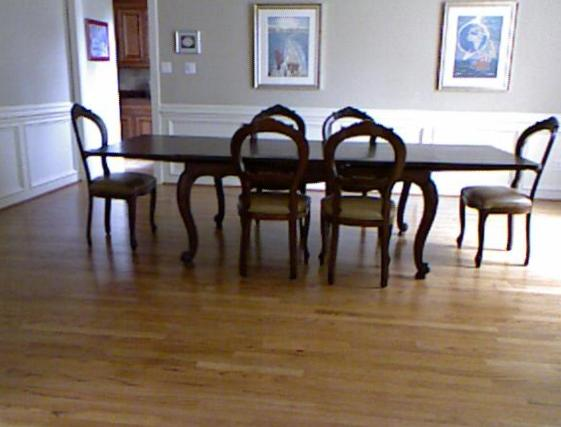
\includegraphics[width=\linewidth]{Figuras/rgb_pre_filling.jpg} 
        \caption{Imagen RGB de cámara}
        \label{fig:img1}
    \end{subfigure}
    \hfill
    \begin{subfigure}[b]{0.32\linewidth}
        \centering
        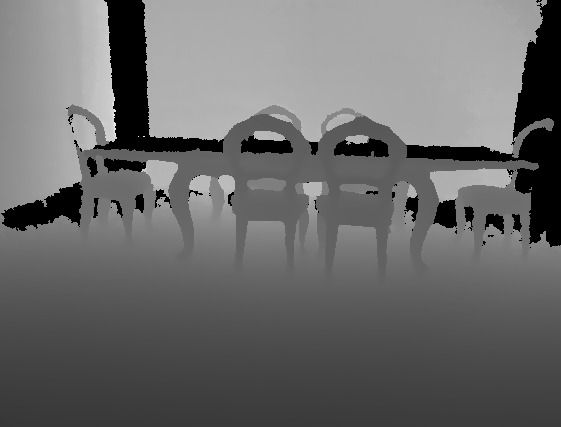
\includegraphics[width=\linewidth]{Figuras/pre_filling.jpg}
        \caption{Profundidad parcial}
        \label{fig:img2}
    \end{subfigure}
    \hfill
    \begin{subfigure}[b]{0.32\linewidth}
        \centering
        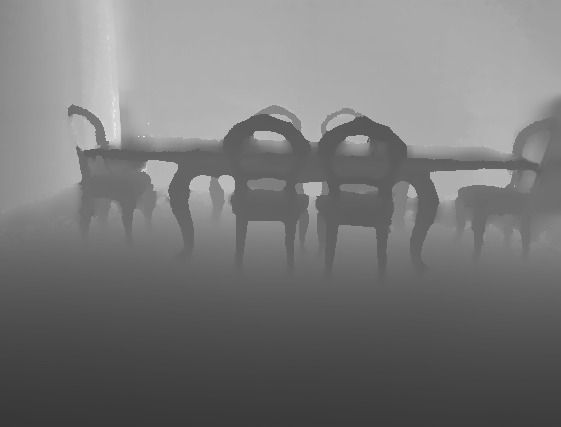
\includegraphics[width=\linewidth]{Figuras/post_filling.jpg}
        \caption{Profundidad rellenada}
        \label{fig:img3}
    \end{subfigure}
    \caption{Comparación de las tres etapas del procesamiento de profundidad. \cite{SUN-RGBD-DATASET-PAPER}}
    \label{fig:comparacion_tres}
\end{figure}

\section{Segmentación Semántica y Filtrado de Objetos}

Disponer de una profundidad densa obtenida mediante el Efficient-UNet resuelve el problema geométrico, pero no el de la comprensión semántica de la escena. Si durante la captura de datos una persona atraviesa el campo de visión de la cámara, o existen objetos dinámicos irrelevantes en el entorno, el algoritmo de odometría los utilizaría como puntos de referencia, introduciendo errores en la trayectoria global. Para evitar este problema, se implementó un filtro semántico basado en el modelo \textbf{YOLO11x-seg}.

No obstante, la integración de este modelo presentó un desafío técnico derivado de la naturaleza óptica del hardware seleccionado.

\subsection{El Problema del Dominio Óptico (RGB a Infrarrojo)}

El modelo YOLO11x-seg fue preentrenado con imágenes a color del conjunto de datos SUN RGB-D para reconocer 17 clases de objetos de interiores. El problema emergió al intentar aplicar este modelo directamente sobre las capturas de la cámara RealSense: el modelo original era incapaz de detectar ningún objeto.

Esta incapacidad responde al fenómeno conocido como \textit{gap} de dominio. El sensor infrarrojo captura intensidades de reflectividad, no luz visible; por lo tanto, las texturas, el patrón de ruido del sensor y la distribución de sombras en una imagen IR son fundamentalmente distintos a los de una fotografía convencional. Resultaba indispensable realizar un proceso de reentrenamiento (\textit{fine-tuning}) para que el modelo aprendiera a operar en el dominio infrarrojo.

\subsection{Generación Automática de Pseudo-Etiquetas (FastSAM)}

Para reentrenar YOLO, era necesario disponer de anotaciones que indicaran la ubicación de los objetos en las 319 imágenes infrarrojas. En lugar de trazar polígonos manualmente para cada fotograma ---un proceso tedioso y propenso a errores humanos---, se desarrolló un script de anotación automática. Para ello se empleó el modelo \textbf{FastSAM} \cite{zhao2023fastsam}, una variante optimizada de \textit{Segment Anything Model} (SAM) que prioriza la velocidad de inferencia y es capaz de procesar las 319 imágenes en menos de dos minutos sin requerir anotación manual. El proceso automatizado siguió los siguientes pasos:

\begin{enumerate}
    \item \textbf{Detección Inicial:} Se ejecutó FastSAM sobre las imágenes IR, replicando el canal de grises para simular una entrada de color y así habilitar la inferencia del modelo.
    \item \textbf{Filtro de Profundidad (Depuración por Umbral de Distancia):} FastSAM tiende a detectar superficies de fondo (paredes distantes) como objetos de interés. Para solucionar esto, las máscaras 2D detectadas se cruzaron con el mapa de profundidad real: si la profundidad promedio de una máscara superaba el percentil 80 de la escena, el script la descartaba automáticamente. Este umbral se seleccionó bajo la premisa operativa de que el mobiliario de interés se encuentra en el 80\% más cercano de la distribución de profundidad de una habitación típica, mientras que el 20\% restante corresponde al fondo y las paredes.
    
    Para validar la selección del percentil 80, se realizó una ablación básica comparando los umbrales 70, 80 y 90 sobre las 318 imágenes capturadas. La Tabla \ref{tab:ablacion_percentil} resume las métricas obtenidas.
    
    \begin{table}[H]
    \centering
    \caption{Ablación del Percentil de Profundidad para Filtrado de FastSAM}
    \label{tab:ablacion_percentil}
    \begin{tabular}{lccc}
    \toprule
    \textbf{Percentil} & \textbf{Mask Ratio Mean} & \textbf{Mask Ratio Min} & \textbf{Mask Ratio Max} \\
    \midrule
    70 (demasiado permisivo) & 91.15\% & 0.52\% & 98.02\% \\
    80 (seleccionado) & 69.88\% & 0.00\% & 97.95\% \\
    90 (demasiado restrictivo) & 61.53\% & 0.00\% & 97.95\% \\
    \bottomrule
    \end{tabular}
    \end{table}
    
    El análisis de la Tabla \ref{tab:ablacion_percentil} revela que el percentil 70 es demasiado permisivo: incluye paredes traseras, cuadros y estanterías como objetos de interés, con lo que incumple la premisa de separar mobiliario cercano del fondo lejano. Por el contrario, el percentil 90 es demasiado restrictivo: descarta mobiliario real (como la cabecera de la cama y la colcha) generando máscaras vacías en algunos fotogramas. El percentil 80 ofrece el balance óptimo: elimina correctamente el fondo lejano y las paredes, mientras conserva el mobiliario de interés en el primer plano. Esta validación básica, aunque limitada a las 318 imágenes del entorno capturado, proporciona evidencia empírica de que la selección del percentil 80 no fue arbitraria. No obstante, la generalización a habitaciones con distribuciones de profundidad atípicas (salas con techos muy altos, pasillos estrechos o espacios abiertos) no fue evaluada y representa una limitación metodológica.

    Es importante destacar que el percentil 80 es un \textbf{parámetro fijo global} aplicado uniformemente a todos los fotogramas, independientemente de las dimensiones del espacio capturado. Este enfoque no escala con el tamaño de la habitación: en una habitación pequeña (p. ej., un pasillo estrecho de 2 m de profundidad), el percentil 80 podría ubicarse a 1.6 m y descartaría erróneamente mobiliario real como objetos de fondo; en una sala grande (p. ej., un salón con doble altura de 10 m de profundidad), el percentil 80 podría ubicarse a 8 m y permitiría que paredes lejanas sean segmentadas como objetos de interés. Esta falta de adaptabilidad impide inherentemente la generalización a distribuciones de profundidad atípicas. La solución robusta sería reemplazar el umbral fijo por un \textbf{criterio adaptativo} basado en estadísticas de la escena (p. ej., la mediana de profundidad del fotograma, el rango intercuartílico o un percentil relativo a la profundidad máxima estimada por el sensor). La implementación de un mecanismo de umbral adaptativo se identifica como \textbf{trabajo futuro} para mejorar la robustez del sistema en escenarios con geometrías distintas a las evaluadas.
    \item \textbf{Formateo de Etiquetas:} Las máscaras supervivientes se suavizaron y se almacenaron en archivos de texto con coordenadas poligonales normalizadas, bajo una única clase unificada: ``Objeto'' (\texttt{class\_id = 0}).
\end{enumerate}

\subsection{Ajuste Fino en Infrarrojo (\textit{Fine-Tuning})}

Con el conjunto de datos etiquetado automáticamente mediante pseudo-etiquetas, se procedió al reentrenamiento de la segmentación de YOLO en el dominio infrarrojo. Para garantizar un aprendizaje correcto, fue necesario modificar sustancialmente la configuración de aumento de datos estándar de Ultralytics:

La selección de hiperparámetros para este \textit{fine-tuning} se fundamentó en el principio de \textbf{transferibilidad de características} establecido por \cite{yosinski2014transferable}: las capas iniciales de una red convolucional aprenden detectores de características generales (bordes, esquinas, texturas) que son transferibles entre dominios, mientras que las capas superiores se especializan en el dominio de entrenamiento original. Con base en este principio, se utilizó una \textbf{tasa de aprendizaje 20 veces menor} que la del entrenamiento original (\texttt{lr0 = 0.0005} frente a \texttt{0.01}) para preservar los pesos del \textit{backbone} preentrenado sin destruir el conocimiento adquirido en SUN RGB-D. Asimismo, se reemplazó el optimizador SGD por \textbf{AdamW}, cuyo mecanismo de tasas adaptativas por parámetro permite una convergencia más rápida y estable en escenarios de \textit{fine-tuning} con conjuntos de datos limitados (319 imágenes).

\begin{itemize}
    \item \textbf{Desactivación de Variaciones de Color:} Se anularon las modificaciones de matiz (\textit{hue}) y saturación (\texttt{hsv\_h = 0.0}, \texttt{hsv\_s = 0.0}), dado que las imágenes infrarrojas carecen de información cromática. Mantener estas transformaciones habría introducido ruido matemático irrelevante durante el entrenamiento.
    \item \textbf{Variación de Intensidad:} Se conservó únicamente una variación moderada de brillo (\texttt{hsv\_v = 0.2}) para que el modelo adquiriera robustez ante las diferencias de exposición generadas por el emisor láser del sensor.
    \item \textbf{Protección de Pseudo-Etiquetas:} Dado que las etiquetas fueron generadas por un modelo de IA (FastSAM) y no por anotadores humanos, contenían un margen de error inherente. Para evitar que el optimizador \texttt{AdamW} se viera afectado negativamente durante el aprendizaje, se redujo el efecto de mosaico a la mitad (\texttt{mosaic = 0.5}) y se desactivó por completo la mezcla de imágenes (\texttt{mixup = 0.0}).
\end{itemize}

Tras 60 épocas de entrenamiento, el resultado fue un modelo YOLO capaz de segmentar el mobiliario directamente desde la señal infrarroja cruda. Las máscaras generadas se envían al algoritmo de odometría para que el cálculo espacial ignore las regiones problemáticas o dinámicas de la escena.

\textbf{Nota sobre la calidad de las pseudo-etiquetas:} Las etiquetas utilizadas para el ajuste fino fueron generadas automáticamente por FastSAM, sin validación manual posterior. La única métrica indirecta de su calidad es que el modelo YOLO reentrenado alcanzó mAP50 = 0.890 sobre ese mismo conjunto, lo cual sugiere consistencia interna. Sin embargo, al no existir comparación contra anotaciones humanas (\textit{ground truth}), no es posible cuantificar el sesgo que estas pseudo-etiquetas pudieron introducir en el proceso de aprendizaje. Una validación manual de una muestra representativa del conjunto de datos quedaría como trabajo futuro para reforzar la solidez metodológica de esta etapa.

\begin{figure}[H]
    \centering
    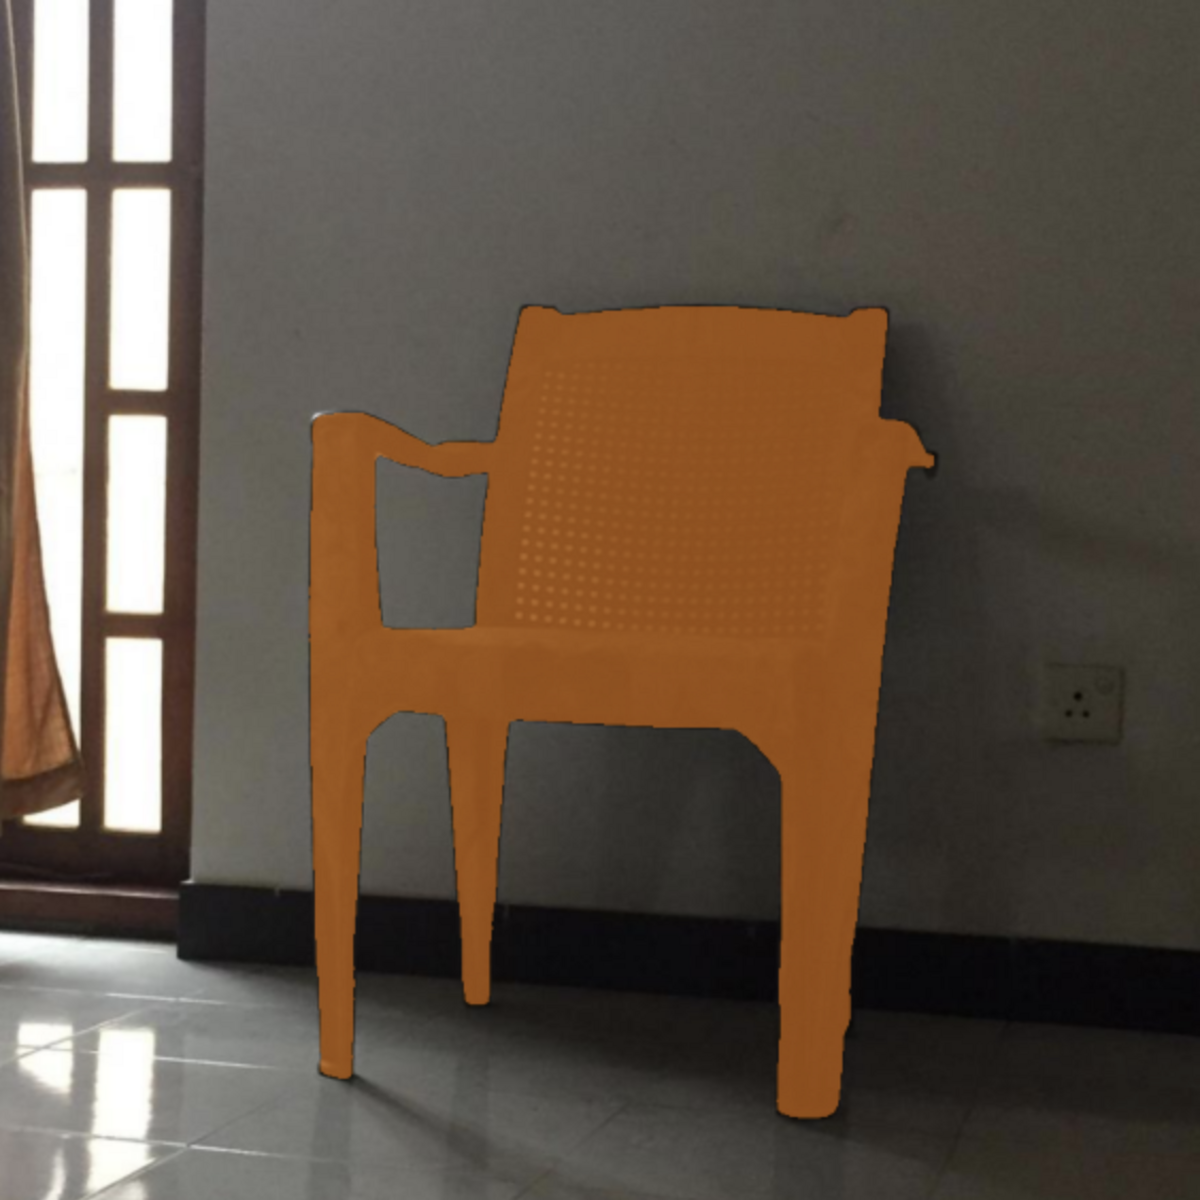
\includegraphics[width=0.6\linewidth]{Figuras/segmentacion_example.png}
    \caption{Ejemplo de segmentación semántica con el modelo YOLO11x-seg sobre imagen infrarroja.}
    \label{fig:yolo_ejemplo}
\end{figure}

\section{Calibración y Registro Intrínseco de la Cámara}

La calibración óptica del sensor es un procedimiento estándar en sistemas de reconstrucción 3D. En este trabajo se optó por extraer los parámetros intrínsecos reales directamente de los archivos de metadatos (\texttt{.csv}) generados por el sensor D430 durante la captura, en lugar de utilizar valores genéricos de fábrica.

Este procedimiento permite que el software conozca el centro óptico y la distancia focal de la lente (\texttt{fx}, \texttt{fy}, \texttt{cx}, \texttt{cy}) específicos de la unidad empleada, lo que mejora la precisión de la proyección de píxeles al espacio tridimensional. Aunque no constituye una aportación metodológica en sí misma, su inclusión explícita evita una fuente común de error sistemático en reconstrucciones con sensores de bajo costo.

\section{Limpieza Geométrica y Eliminación de Valores Atípicos}

Tras el relleno de profundidad con la red neuronal, el sensor puede generar ruido residual en los bordes de los objetos, manifestado como puntos aislados o flotantes que no corresponden a ninguna superficie real. Para eliminar estos artefactos antes de la fusión volumétrica final, se implementó un filtro de eliminación estadística de valores atípicos (\textit{Statistical Outlier Removal}).

El algoritmo analiza cada punto de la nube y calcula su distancia promedio hacia sus vecinos más cercanos. Si un punto se encuentra excesivamente alejado del grupo vecinal en función de un umbral de desviación estándar configurado, el sistema lo clasifica como ruido del sensor y lo elimina automáticamente. Este paso es fundamental para que las superficies del gemelo digital presenten continuidad geométrica, evitando picos o discontinuidades causados por lecturas erróneas del sensor.

\section{Proceso de Odometría e Integración Volumétrica}

Con los fotogramas depurados y calibrados, el sistema procede a integrarlos en un modelo tridimensional unificado. El método de integración se articula en dos etapas lógicas:

\begin{itemize}
    \item \textbf{Alineación Híbrida (ICP punto-a-plano):} Para estimar el movimiento de la cámara, se empleó un esquema que combina la intensidad de la imagen con la geometría del mapa de profundidad. El sistema utiliza las normales de las superficies para alinear los fotogramas de manera progresiva, rechazando automáticamente aquellos intentos de alineación que no alcancen un umbral mínimo de confianza (\textit{Fitness}).
    \item \textbf{Fusión en Volumen TSDF:} En lugar de acumular puntos de forma directa, se emplea una cuadrícula volumétrica de vóxeles de alta resolución. Cada vez que la cámara observa una superficie, el sistema actualiza los vóxeles correspondientes promediando las mediciones sucesivas, lo que permite cancelar el ruido temporal y modelar una superficie sólida de forma progresiva. Este método constituye el estándar de referencia para la fusión de mapas de profundidad en tiempo real \cite{curless1996volumetric}.
\end{itemize}

Como estrategia de validación indirecta del error acumulado global, se implementó un análisis de consistencia geométrica posterior a la reconstrucción. Este análisis, descrito en la Sección \ref{sec:consistencia}, extrae los planos dominantes de la malla final mediante RANSAC y evalúa la ortogonalidad, paralelismo y perpendicularidad de las superficies arquitectónicas. Aunque no sustituye a un \textit{ground truth} de trayectoria externo, permite cuantificar el \textit{drift} estructural como proxy de la calidad global del gemelo digital.

\section{Post-procesamiento y Optimización de la Malla}

El último paso de la metodología consiste en transformar el volumen generado en un archivo manejable y exportable. Para ello, se extrae la malla poligonal del volumen TSDF y se le aplican dos tratamientos matemáticos secuenciales:

\begin{enumerate}
    \item \textbf{Suavizado de Taubin:} Este filtro fue seleccionado específicamente porque permite eliminar las irregularidades de la superficie sin reducir el volumen real de los objetos, preservando así las dimensiones métricas de la habitación \cite{taubin1995signal}.
    \item \textbf{Simplificación por Decimación:} Dado que la fusión volumétrica genera millones de polígonos redundantes, especialmente en zonas planas como paredes y suelo, se aplicó un algoritmo de decimación cuadrática basado en \textit{Quadric Error Metrics} \cite{garland1997surface}. Este proceso colapsa los triángulos de pequeña dimensión en regiones uniformes, conservando el detalle geométrico únicamente donde es estructuralmente relevante, y produciendo como resultado un archivo ligero y compatible con cualquier software de diseño o visualización 3D.
\end{enumerate}

\chapter{Resultados}

En este capítulo se presentan los resultados experimentales obtenidos tras la ejecución de la metodología propuesta. El análisis se organiza en torno al rendimiento de sus tres componentes: el modelo de completado de profundidad (Efficient-UNet), el filtro de segmentación semántica (YOLO11x-seg) y la precisión geométrica de la reconstrucción volumétrica final. Cada componente fue evaluado de forma independiente; la integración completa se evaluó sobre una secuencia de 338 fotogramas capturados en un único entorno interior, de los cuales 319 fueron integrados exitosamente tras la validación por ICP.

Antes de detallar los resultados, es necesario establecer una distinción metodológica fundamental sobre las métricas reportadas en este capítulo. No todas las métricas poseen el mismo nivel de validación externa. La Tabla \ref{tab:tipos_validacion} clasifica las métricas principales según el tipo de referencia de verdad (\textit{ground truth}) empleada.

\begin{table}[H]
\centering
\caption{Clasificación de Métricas por Tipo de Validación}
\label{tab:tipos_validacion}
\resizebox{\textwidth}{!}{%
\begin{tabular}{p{3.5cm}p{3.5cm}p{4.5cm}p{4.5cm}}
\toprule
\textbf{Métrica} & \textbf{Componente} & \textbf{Tipo de Validación} & \textbf{Referencia de Verdad} \\
\midrule
MAE, RMSE, $\delta < 1.25$ & Efficient-UNet & \textbf{Validación externa} & Mapas de profundidad reales del sensor (SUN RGB-D + capturas propias) \\
\midrule
Box mAP50, Mask mAP50 & YOLO11x-seg & \textbf{Consistencia interna} & Pseudo-etiquetas generadas por FastSAM (mismo conjunto de entrenamiento) \\
\midrule
ICP Fitness, ICP RMSE & Odometría visual & \textbf{Validación externa} & Correspondencias geométricas entre fotogramas consecutivos \\
\midrule
Ortogonalidad, paralelismo, escala métrica & Malla final (TSDF) & \textbf{Validación indirecta} & Propiedades arquitectónicas teóricas + medición física con cinta métrica \\
\bottomrule
\end{tabular}%
}
\end{table}

La distinción de la Tabla \ref{tab:tipos_validacion} es crucial para interpretar correctamente los resultados. Las métricas de Efficient-UNet y de odometría ICP fueron evaluadas contra datos de referencia reales: mapas de profundidad capturados por el sensor y correspondencias geométricas entre fotogramas. En contraste, el mAP de YOLO11x-seg es una métrica de \textit{consistencia interna}: el modelo se validó contra el mismo conjunto de pseudo-etiquetas que se utilizó para su entrenamiento, sin anotación humana independiente. Por tanto, el mAP de YOLO no es comparable con valores reportados en trabajos que validan contra \textit{ground truth} humano, y debe interpretarse como una medida de estabilidad del aprendizaje, no como una validación de precisión absoluta de segmentación.

\section{Evaluación y Selección del Modelo de Completado de Profundidad}

El primer componente crítico del \textit{pipeline} es la red neuronal encargada de estimar la información faltante en las lecturas del sensor infrarrojo. Para justificar la selección de la arquitectura final y validar su impacto en la reconstrucción, se realizó un estudio comparativo evaluando tres iteraciones del modelo de aprendizaje profundo sobre un conjunto de validación independiente de 1{,}399 imágenes.

Las arquitecturas evaluadas fueron:
\begin{itemize}
    \item \textbf{ResNet18 (Línea Base):} Un modelo Encoder-Decoder estándar utilizado como punto de partida para evaluar la viabilidad de la tarea.
    \item \textbf{Efficient-UNet (V1):} Se sustituyó el codificador por EfficientNet-B0 para mejorar la extracción de características, utilizando una función de pérdida estándar (L1/MSE).
    \item \textbf{Efficient-UNet (V2 - Propuesto):} La arquitectura definitiva, la cual integra la función personalizada \textit{Edge-Aware Loss} para penalizar el difuminado geométrico en los bordes de los objetos.
\end{itemize}

El análisis se estructuró en dos fases: una evaluación métrica sobre la escena completa y una evaluación crítica centrada en las zonas donde el sensor físico falló (huecos).

\subsection{Estudio Comparativo: Evaluación Global}

En esta primera prueba se midió la diferencia matemática entre las predicciones y los mapas de profundidad reales (\textit{Ground Truth}) sobre el área total de cada fotograma. Los resultados obtenidos se resumen en la Tabla \ref{tab:depth_global_metrics}.

\begin{table}[H]
\centering
\caption{Rendimiento global comparativo de los modelos de profundidad.}
\label{tab:depth_global_metrics}
\resizebox{\textwidth}{!}{%
\begin{tabular}{lccc}
\toprule
\textbf{Métrica} & \textbf{ResNet18 (Base)} & \textbf{Efficient-UNet (V1)} & \textbf{Efficient-UNet (V2)} \\
\midrule
Precisión Fina ($\delta < 1.25$)     & 93.57\% & 98.14\% & \textbf{98.33\%} \\
Precisión Media ($\delta < 1.25^2$)  & 97.76\% & 99.29\% & \textbf{99.31\%} \\
Precisión Gruesa ($\delta < 1.25^3$) & 99.11\% & \textbf{99.58\%} & 99.56\% \\
Error Absoluto Medio (MAE)           & 0.1797 m & 0.0716 m & \textbf{0.0664 m} \\
Error Cuadrático Medio (RMSE)        & 0.3777 m & \textbf{0.2158 m} & 0.2227 m \\
\bottomrule
\end{tabular}%
}
\end{table}

Los resultados globales demuestran la necesidad de escalar la arquitectura inicial. El modelo ResNet18 obtuvo un Error Absoluto Medio (MAE) de casi 18 centímetros, lo cual resulta inadecuado para una reconstrucción arquitectónica. La transición a Efficient-UNet (V1) redujo este error a 7.1 cm. 

Es fundamental destacar el comportamiento del Modelo V2: aunque registra un RMSE ligeramente superior al del Modelo V1 (0.2227 m vs 0.2158 m), logra la mejor precisión fina (98.33\%) y el menor error absoluto (6.6 cm). Este comportamiento es una validación directa de la función \textit{Edge-Aware Loss}; mientras que el Modelo V1 minimiza el RMSE mediante un suavizado general de la escena, el Modelo V2 prioriza la nitidez de los bordes, generando transiciones geométricas más realistas que penalizan ligeramente la métrica cuadrática pero mejoran la fidelidad estructural.

\subsection{Evaluación Crítica: Rendimiento en Zonas Ciegas (Huecos)}

Para medir la capacidad inferencial de la red neuronal, se aisló la evaluación excluyendo las áreas con información válida y midiendo el error \textit{únicamente} en los huecos del sensor (más de 85 millones de píxeles evaluados para el modelo final).

\begin{table}[H]
\centering
\caption{Rendimiento inferencial del modelo (Exclusivo en Zonas Ciegas/Huecos).}
\label{tab:depth_holes_metrics}
\resizebox{\textwidth}{!}{%
\begin{tabular}{lccc}
\toprule
\textbf{Métrica} & \textbf{ResNet18 (Base)} & \textbf{Efficient-UNet (V1)} & \textbf{Efficient-UNet (V2)} \\
\midrule
Precisión Fina ($\delta < 1.25$)     & 76.91\% & 91.47\% & \textbf{92.47\%} \\
Precisión Media ($\delta < 1.25^2$)  & 90.81\% & 96.60\% & \textbf{96.73\%} \\
Precisión Gruesa ($\delta < 1.25^3$) & 95.95\% & \textbf{97.97\%} & 97.86\% \\
Error Absoluto Medio (MAE)           & 0.4316 m & 0.2256 m & \textbf{0.2179 m} \\
Error Cuadrático Medio (RMSE)        & 0.7466 m & \textbf{0.4954 m} & 0.5080 m \\
\bottomrule
\end{tabular}%
}
\end{table}

El análisis de las zonas ciegas justifica concluyentemente las decisiones metodológicas. El modelo ResNet18 presentó un colapso en su capacidad inferencial, logrando apenas un 76.91\% de precisión fina y un error promedio superior a 43 centímetros. Alimentar al algoritmo de odometría con desviaciones de esta magnitud generaría una trayectoria errática.

Por el contrario, el modelo propuesto (V2) elevó la precisión fina en los huecos al 92.47\%. Al igual que en la evaluación global, se mantiene la tendencia donde el Modelo V2 mejora el MAE y la precisión respecto al V1, a pesar de la ligera penalización en el RMSE. Esta capacidad de inferir la profundidad con un margen de 21.7 cm en ausencia total de datos de referencia permite sellar los vacíos estructurales del mapa, proporcionando superficies continuas indispensables para el anclaje del algoritmo ICP en la etapa de reconstrucción.

\subsubsection{Registro de Entrenamiento y Curvas de Convergencia}

A diferencia del módulo de segmentación semántica, el entrenamiento del modelo Efficient-UNet no generó archivos de registro histórico (logs de pérdida por época) debido a que el proceso de preentrenamiento y ajuste fino se ejecutó en un entorno de desarrollo interactivo donde las métricas se reportaron únicamente en la consola estándar. En consecuencia, no fue posible reconstruir a posteriori las curvas de aprendizaje del completado de profundidad. Sin embargo, las métricas finales de validación reportadas en las Tablas \ref{tab:depth_global_metrics} y \ref{tab:depth_holes_metrics} fueron obtenidas de manera rigurosa sobre un conjunto de validación independiente de 1{,}399 imágenes, garantizando que los valores reportados (RMSE, MAE, precisión $\delta < 1.25$) reflejan el estado de convergencia del modelo al final del entrenamiento.

Como trabajo futuro, se recomienda instrumentar el script de entrenamiento para persistir las métricas por época en un archivo CSV o TensorBoard, lo que permitiría analizar la velocidad de convergencia, detectar sobreajuste temprano y comparar el comportamiento de la función \textit{Edge-Aware Loss} frente a la pérdida L1 estándar a lo largo del tiempo.

\subsubsection{Ejemplos Visuales}

\begin{figure}[H]
    \centering
    \begin{subfigure}[b]{0.95\linewidth}
        \centering
        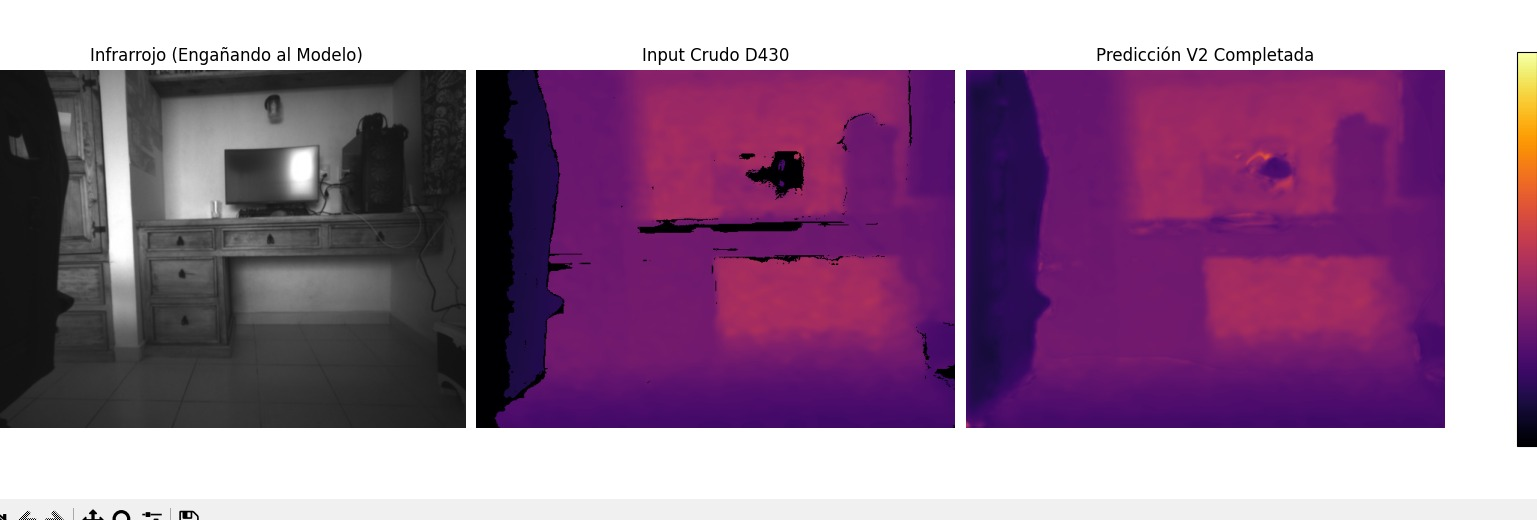
\includegraphics[width=\linewidth]{Figuras/Depth_Ex.jpeg} 
        \label{fig:depth_ex1}
    \end{subfigure}
    
    \vspace{0.5cm}
    
    \begin{subfigure}[b]{0.95\linewidth}
        \centering
        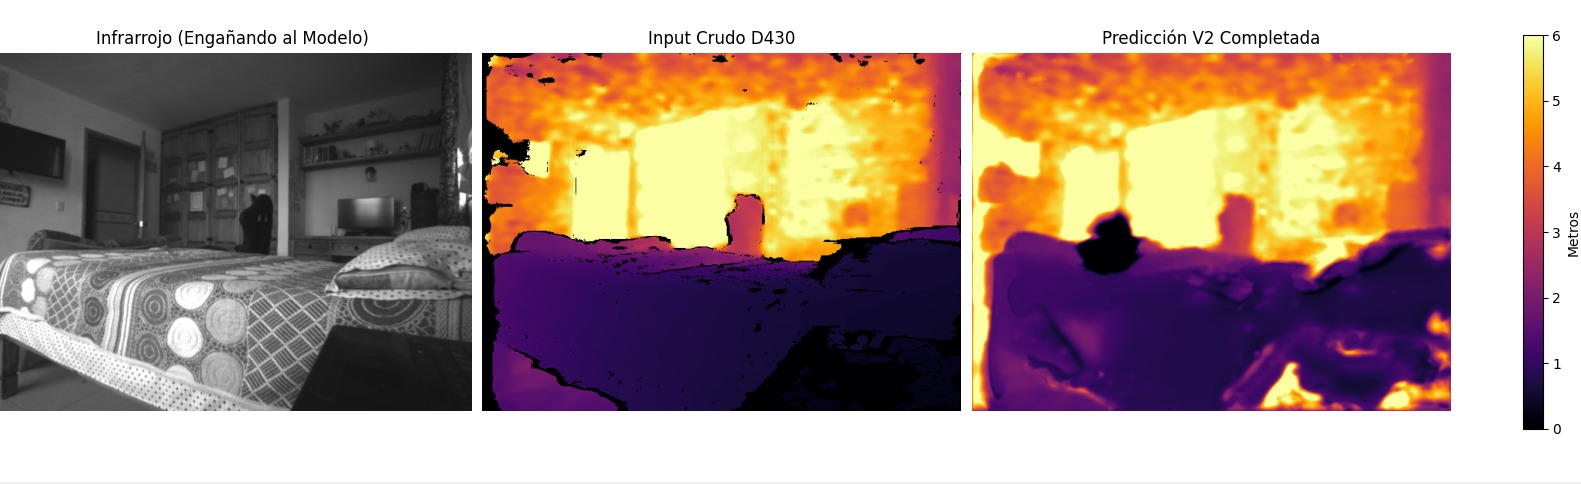
\includegraphics[width=\linewidth]{Figuras/Depth_Ex_2.jpeg}
        \label{fig:depth_ex2}
    \end{subfigure}
    \caption{Ejemplos de relleno de profundidad estimado sobre la base de datos SUN RGB-D. \cite{SUN-RGBD-DATASET-PAPER}}
    \label{fig:depth_examples}
\end{figure}

\section{Resultados de la Segmentación Semántica (YOLO11x-seg)}

El segundo componente de la arquitectura propuesta es la capacidad del sistema para comprender semánticamente la escena que observa. Tal como se detalló en la metodología, el modelo YOLO11x-seg fue adaptado para operar exclusivamente en el espectro infrarrojo (IR). Su objetivo es clasificar y segmentar los elementos de la escena, diferenciando la estructura estática (paredes y suelo) de los elementos volumétricos complejos (mobiliario), lo cual resulta crucial para un filtrado inteligente durante la etapa de odometría.

Tras el proceso de entrenamiento y ajuste fino (\textit{fine-tuning}), el modelo fue sometido a validación, obteniéndose las métricas globales y por clase que se presentan a continuación.

\subsection{Precisión Global de Detección y Segmentación}

El rendimiento general del modelo mostró resultados positivos, indicando que el ajuste fino fue suficiente para que la arquitectura operara sobre el espectro infrarrojo. Sin embargo, dado que la validación se realizó sobre el mismo conjunto de pseudo-etiquetas generadas por FastSAM, estos resultados reflejan principalmente la consistencia del modelo respecto a su propio conjunto de entrenamiento, y no necesariamente su desempeño sobre anotaciones humanas independientes.

\begin{table}[H]
\centering
\caption{Métricas Globales de Validación (YOLO11x-seg en Infrarrojo)}
\label{tab:yolo_global}
\begin{tabular}{lc}
\toprule
\textbf{Métrica de Evaluación} & \textbf{Resultado} \\
\midrule
Box mAP50 (Precisión de Detección) & 0.9000 (90.00\%) \\
Box mAP50-95 & 0.7720 (77.20\%) \\
Mask mAP50 (Precisión de Máscara) & 0.8782 (87.82\%) \\
Mask mAP50-95 & 0.6525 (65.25\%) \\
\bottomrule
\end{tabular}
\end{table}

Alcanzar un 90.00\% en la detección de cajas delimitadoras (Box mAP50) y un 87.82\% en la generación de máscaras (Mask mAP50) indica que el modelo aprendió a segmentar los objetos de interés en el dominio infrarrojo. Nuevamente, es necesario interpretar estos valores con cautela, dado que fueron calculados sobre el mismo conjunto de pseudo-etiquetas utilizado para el ajuste fino, sin validación cruzada con anotaciones independientes.

\subsection{Análisis Semántico por Clase}

Para que la reconstrucción tridimensional sea verdaderamente versátil, resulta necesario evaluar el comportamiento del modelo frente a las tres categorías fundamentales del entorno físico interior: paredes (\textit{wall}), suelo (\textit{floor}) y mobiliario (\textit{furniture}).

\begin{table}[H]
\centering
\caption{Rendimiento de Segmentación (Mask AP) Desglosado por Clase}
\label{tab:yolo_classes}
\begin{tabular}{lcc}
\toprule
\textbf{Categoría Semántica} & \textbf{AP50} & \textbf{AP (mAP50-95)} \\
\midrule
Suelo (\textit{floor}) & 0.9467 (94.67\%) & 0.7227 (72.27\%) \\
Mobiliario (\textit{furniture}) & 0.8959 (89.59\%) & 0.6517 (65.17\%) \\
Pared (\textit{wall}) & 0.7919 (79.19\%) & 0.5830 (58.30\%) \\
\bottomrule
\end{tabular}
\end{table}

El análisis por clase revela los siguientes hallazgos:

\begin{itemize}
    \item \textbf{Suelo (94.67\%):} Obtuvo la precisión más alta de las tres categorías. Al tratarse de una superficie continua y generalmente perpendicular al eje inferior de captura de la cámara, el proyector infrarrojo genera un patrón de retorno estable y uniforme, lo que permite a la red identificar el suelo con alta consistencia.
    \item \textbf{Mobiliario (89.59\%):} Representa los objetos volumétricos de interés en la escena (mesas, sillas, estantes). Un rendimiento cercano al 90\% garantiza que el sistema puede aislar de forma sistemática estos elementos complejos, lo que en el futuro permitirá aplicarles reglas físicas diferenciadas o excluirlos selectivamente de la odometría estática.
    \item \textbf{Paredes (79.19\%):} Presentaron el rendimiento más bajo, resultado que resulta coherente con las características del sensor. En el espectro infrarrojo, una pared lisa y distante carece de bordes texturizados diferenciables, lo que provoca que su señal se difumine con las esquinas oscuras o las zonas fuera del alcance del proyector. A pesar de ello, un 79\% sigue constituyendo un margen suficientemente robusto para establecer de forma confiable los límites espaciales de la habitación.
\end{itemize}

\subsection{Ejemplos Visuales}

\begin{figure}[H]
    \centering
    \begin{subfigure}[b]{0.32\linewidth}
        \centering
        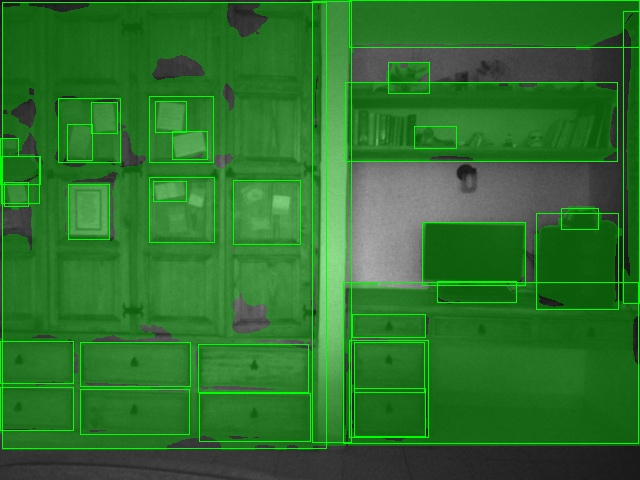
\includegraphics[width=\linewidth]{Figuras/segmentacion_ejemplo_0.jpeg} 
        \label{fig:seg_ex1}
    \end{subfigure}
    \hfill
    \begin{subfigure}[b]{0.32\linewidth}
        \centering
        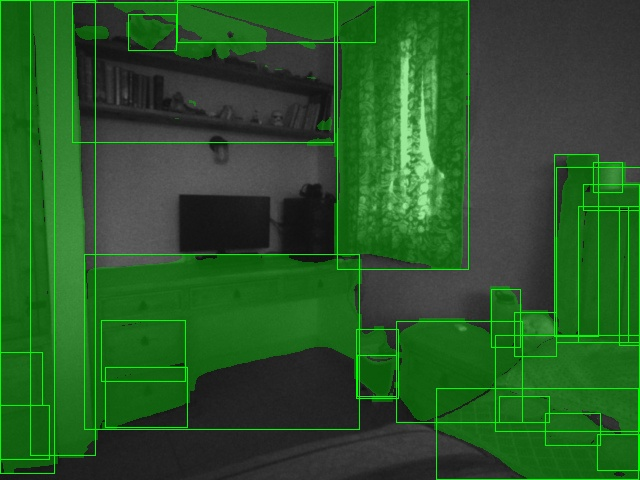
\includegraphics[width=\linewidth]{Figuras/segmentacion_ejemplo_1.jpeg}
        \label{fig:seg_ex2}
    \end{subfigure}
    \hfill
    \caption{Ejemplos de segmentación semántica con YOLO11x-seg sobre imágenes infrarrojas.}
    \label{fig:comparacion_seg}
\end{figure}

\section{Resultados de la Reconstrucción 3D y Odometría Visual}

El último paso de la metodología es la integración espacial de toda la información procesada. Tras reparar los mapas de profundidad con la red Efficient-UNet y filtrar semánticamente la escena, el sistema calculó la trayectoria de la cámara y fusionó el entorno físico en un volumen TSDF.

Para esta evaluación final, se procesó una secuencia continua de 338 fotogramas capturados en un entorno interior complejo, de los cuales 319 fueron integrados exitosamente tras la validación por ICP. A diferencia de las pruebas de laboratorio con datos genéricos, el \textit{pipeline} extrajo y aplicó los parámetros intrínsecos reales de la cámara registrados durante la grabación (distancia focal $f_x = 380.69$, $f_y = 380.69$ y centro óptico $c_x = 317.98$, $c_y = 235.06$). Esto garantizó que las métricas de error reflejaran el comportamiento físico exacto del sensor D430 y no una aproximación del software.

\subsection{Precisión de la Trayectoria (Métricas ICP)}

La fiabilidad de un gemelo digital depende de que la cámara no acumule errores de posición durante su desplazamiento por el espacio. Las métricas arrojadas por el algoritmo de alineación (ICP punto-a-plano) a lo largo de toda la secuencia demostraron una estabilidad notable:

\begin{table}[H]
\centering
\caption{Métricas de Odometría Visual e Integración (319 fotogramas integrados)}
\label{tab:reconstruction_metrics}
\begin{tabular}{lc}
\toprule
\textbf{Métrica de Evaluación} & \textbf{Resultado Promedio} \\
\midrule
Proporción de Profundidad Válida (\textit{Valid Depth}) & 92.35\% \\
Nivel de Ajuste Geométrico (\textit{ICP Fitness}) & 95.54\% \\
Error Cuadrático Medio de Alineación (\textit{ICP RMSE}) & 0.0252 m \\
\bottomrule
\end{tabular}
\end{table}

El primer indicador de relevancia es el 92.35\% de profundidad válida. Este resultado confirma el éxito de la etapa de completado de profundidad (Efficient-UNet): al entregar al módulo de odometría fotogramas donde prácticamente la totalidad del área presenta una distancia utilizable, el algoritmo dispone de una mayor superficie de anclaje, previniendo de forma efectiva los fallos de rastreo.

Como resultado de esta disponibilidad de datos, el sistema mantuvo un nivel de ajuste (\textit{Fitness}) del 95.54\%, lo que indica que, en promedio, más de 9 de cada 10 puntos en un fotograma encontraron correspondencia geométrica durante el desplazamiento de la cámara. El Error Cuadrático Medio de alineación fue de \textbf{2.52 centímetros (0.0252 m)} entre empalmes consecutivos. Este resultado es alentador para un sensor de bajo costo, aunque debe interpretarse como el error de alineación local entre fotogramas consecutivos, no como el error acumulado de la trayectoria completa, el cual no fue evaluado con una referencia de \textit{ground truth} externa.

\subsection{Fidelidad y Complejidad de la Malla Volumétrica}

El resultado tangible de todo el proceso es el gemelo digital exportado. El volumen TSDF fue configurado para capturar el entorno con un nivel de detalle milimétrico, generando una representación inicial de extrema fidelidad geométrica. Sin embargo, para un trabajo orientado a aplicaciones prácticas (diseño de interiores, realidad aumentada), el tamaño manejable del archivo final es una métrica tan relevante como la precisión geométrica. La Tabla \ref{tab:complejidad_malla} compara las dimensiones de la malla TSDF original extraída del volumen contra la malla decimada final exportada para uso en software de terceros.

\begin{table}[H]
\centering
\caption{Complejidad y Tamaño de Archivo: Malla TSDF Original vs. Malla Decimada Final}
\label{tab:complejidad_malla}
\resizebox{\textwidth}{!}{%
\begin{tabular}{lccc}
\toprule
\textbf{Métrica} & \textbf{Malla TSDF Original} & \textbf{Malla Decimada Final} & \textbf{Reducción} \\
\midrule
Vértices & 11{,}409{,}829 & 69{,}532 & 99.4\% \\
Triángulos & 14{,}148{,}189 & 150{,}067 & 98.9\% \\
Tamaño de archivo (\texttt{.ply}) & 730.35 MB & 5.24 MB & 99.3\% \\
\bottomrule
\end{tabular}%
}
\end{table}

Las superficies del mobiliario y las paredes se reconstruyeron de forma continua en la malla original, demostrando que el volumen TSDF logró absorber y promediar las ligeras fluctuaciones acumuladas a lo largo de los 319 fotogramas integrados. El proceso de decimación cuadrática basada en \textit{Quadric Error Metrics} \cite{garland1997surface} redujo la complejidad poligonal en un 98.9\% (de 14.1 M a 150 K triángulos), produciendo un archivo de 5.24 MB manejable para importación directa en software de diseño de interiores (SketchUp, Blender) y motores de realidad aumentada (Unity). Cabe destacar que la decimación preservó el detalle estructural en bordes y esquinas, mientras colapsó triángulos redundantes en zonas planas (paredes y suelo), manteniendo la fidelidad métrica del modelo.

\begin{figure}[H]
    \centering
    \begin{subfigure}[c]{0.48\linewidth}
        \centering
        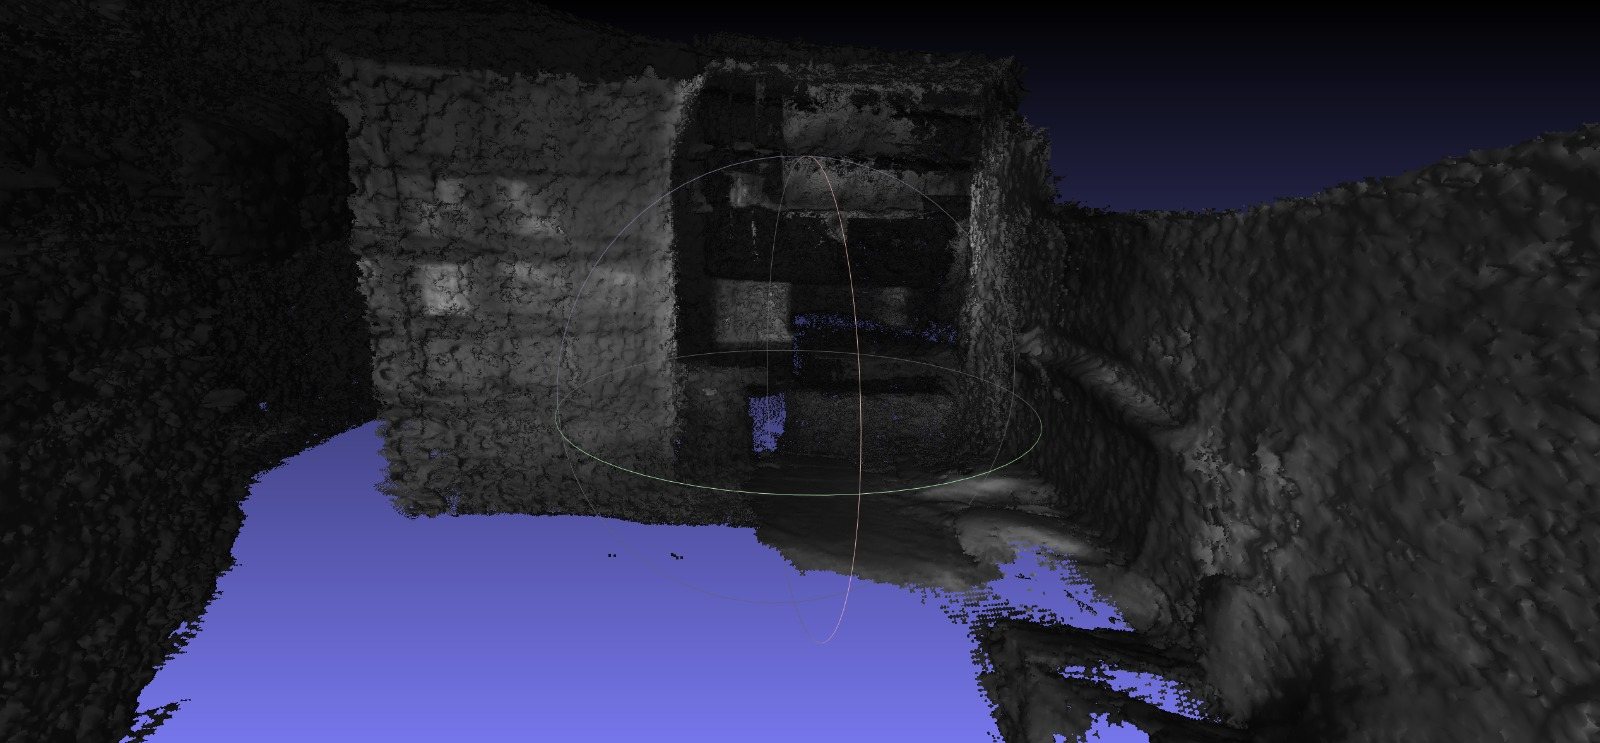
\includegraphics[width=\linewidth, height=5.5cm, keepaspectratio]{Figuras/Reconstruccion 2.jpeg}
        \caption{Vista lateral de la malla TSDF}
        \label{fig:recon2}
    \end{subfigure}
    \hfill
    \begin{subfigure}[c]{0.48\linewidth}
        \centering
        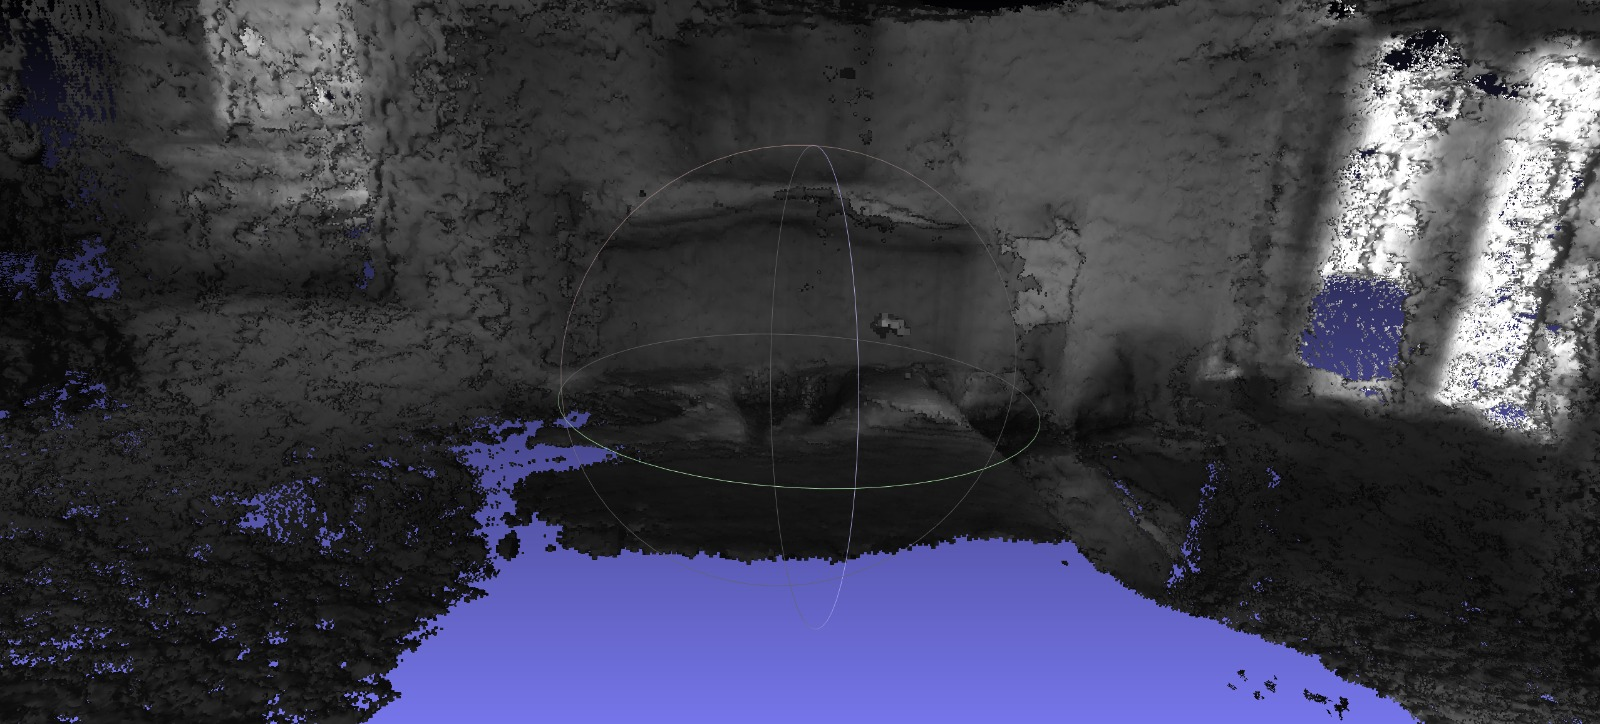
\includegraphics[width=\linewidth, height=5.5cm, keepaspectratio]{Figuras/Reconstrucción 3.jpeg}
        \caption{Vista superior de la habitación reconstruida}
        \label{fig:recon3}
    \end{subfigure}
    \caption{Modelo 3D final de la reconstrucción. La integración TSDF de 319 fotogramas infrarrojos produce una malla geométricamente coherente con superficies continuas.}
    \label{fig:reconstruccion_final}
\end{figure}

La inspección visual detallada de la malla TSDF (Figuras \ref{fig:recon2} y \ref{fig:recon3}) permite realizar una evaluación cualitativa del \textit{drift} acumulado. A nivel macroscópico, la reconstrucción no presenta duplicaciones estructurales severas ni paredes ``fantasma'' (hallazgos comunes en sistemas SLAM con \textit{drift} descontrolado). Las superficies del mobiliario y las paredes mantienen una continuidad geométrica razonable, lo que indica que el sistema logró un cierre local adecuado de la superficie.

No obstante, al examinar las esquinas de la habitación, se aprecian ligeras desalineaciones consistentes con la acumulación de error de rotación. El análisis de consistencia geométrica global (Tabla \ref{tab:consistencia_geometrica}) cuantifica esta observación: las paredes adyacentes presentan desviaciones angulares de hasta $29.41^{\circ}$ respecto a la ortogonalidad teórica, y las paredes opuestas no mantienen el paralelismo esperado. Estas deformaciones son coherentes con el error de alineación local de $2.52$ cm multiplicado por la secuencia de 319 fotogramas, y validan la hipótesis de que el \textit{drift} es el principal factor limitante del sistema en su configuración actual.

\subsection{Análisis de Consistencia Geométrica Global}
\label{sec:consistencia}

El \textit{ATE} (\textit{Absolute Trajectory Error}) es la métrica estándar en benchmarks de SLAM para cuantificar la deriva acumulada de la trayectoria \cite{TUM-RGBD, ICL-NUIM}. Su cálculo requiere un \textit{ground truth} de trayectoria externo, típicamente obtenido mediante un sistema de captura de movimiento o una estación total. Dado que este proyecto utilizó un sensor de bajo costo en un entorno sin infraestructura de referencia, no fue posible obtener dicho \textit{ground truth}. En su lugar, se implementó un análisis de consistencia geométrica global (RANSAC sobre planos de la malla TSDF) como \textbf{proxy del \textit{drift} acumulado}. Esta estrategia está alineada con la literatura de odometría visual auto-supervisada, donde la consistencia geométrica se utiliza como sustituto de la referencia externa cuando el \textit{ground truth} no está disponible \cite{iyer2018geometric}. Trabajos recientes de evaluación sin \textit{ground truth} en SLAM visual reafirman que la consistencia estructural de la reconstrucción es una métrica válida para evaluar la calidad global del sistema en ausencia de referencias de trayectoria \cite{fontan2024look}.

La fiabilidad de un gemelo digital no solo depende de la precisión local del empalme entre fotogramas consecutivos, sino también de la \textit{coherencia estructural global} del modelo tridimensional resultante. Si la trayectoria de la cámara acumula error de posición (fenómeno conocido como \textit{drift}), la malla final exhibirá deformaciones geométricas detectables a nivel arquitectónico: paredes adyacentes que no forman ángulos rectos, paredes opuestas que no son paralelas, o una escala vertical irreal.

Para cuantificar indirectamente la magnitud del \textit{drift} acumulado sin disponer de un \textit{ground truth} de trayectoria externo, se implementó un análisis de consistencia geométrica global sobre la malla TSDF final. Mediante el algoritmo RANSAC (\textit{Random Sample Consensus}) se extrajeron los planos dominantes (paredes, piso y techo) de la nube de puntos integrada. A partir de los modelos de plano $(a, b, c, d)$ se calcularon: (a) los ángulos entre normales de paredes adyacentes (esperado: $90^{\circ}$), (b) el paralelismo de paredes opuestas (esperado: $0^{\circ}$ o $180^{\circ}$), y (c) los ángulos de perpendicularidad entre paredes y el suelo (esperado: $90^{\circ}$).

La Tabla \ref{tab:consistencia_geometrica} resume los resultados obtenidos para la malla final de 319 fotogramas.

\begin{table}[H]
\centering
\caption{Métricas de Consistencia Geométrica Global de la Malla Final}
\label{tab:consistencia_geometrica}
\resizebox{\textwidth}{!}{%
\begin{tabular}{lccc}
\toprule
\textbf{Métrica de Evaluación} & \textbf{Valor Medido} & \textbf{Valor Esperado} & \textbf{Desviación} \\
\midrule
Ángulo Pared 0 -- Pared 1 (adyacentes) & $79.98^{\circ}$ & $90.00^{\circ}$ & $-10.02^{\circ}$ \\
Ángulo Pared 0 -- Pared 3 (adyacentes) & $83.31^{\circ}$ & $90.00^{\circ}$ & $-6.69^{\circ}$ \\
Ángulo Pared 1 -- Pared 2 (adyacentes) & $60.59^{\circ}$ & $90.00^{\circ}$ & $-29.41^{\circ}$ \\
Ángulo Pared 2 -- Pared 3 (adyacentes) & $61.87^{\circ}$ & $90.00^{\circ}$ & $-28.13^{\circ}$ \\
\midrule
Paralelismo Pared 0 -- Pared 2 (opuestas) & $21.58^{\circ}$ & $0.00^{\circ}$ & $+21.58^{\circ}$ \\
Paralelismo Pared 1 -- Pared 3 (opuestas) & $18.33^{\circ}$ & $0.00^{\circ}$ & $+18.33^{\circ}$ \\
\midrule
Ángulo Pared 0 -- Suelo & $88.17^{\circ}$ & $90.00^{\circ}$ & $-1.83^{\circ}$ \\
Ángulo Pared 1 -- Suelo & $77.07^{\circ}$ & $90.00^{\circ}$ & $-12.93^{\circ}$ \\
Ángulo Pared 2 -- Suelo & $87.38^{\circ}$ & $90.00^{\circ}$ & $-2.62^{\circ}$ \\
Ángulo Pared 3 -- Suelo & $84.84^{\circ}$ & $90.00^{\circ}$ & $-5.16^{\circ}$ \\
\midrule
Distancia entre paredes opuestas (Pared 0 -- Pared 2) & $0.036$ m & Variable & --- \\
Distancia entre paredes opuestas (Pared 1 -- Pared 3) & $2.293$ m & Variable & --- \\
\bottomrule
\end{tabular}%
}
\end{table}

Los resultados de la Tabla \ref{tab:consistencia_geometrica} revelan una degradación sistemática de la ortogonalidad arquitectónica en la malla final. Las desviaciones angulares entre paredes adyacentes oscilan entre $6.69^{\circ}$ y $29.41^{\circ}$, lejos del ángulo recto teórico. Asimismo, las paredes opuestas presentan errores de paralelismo de $18.33^{\circ}$ y $21.58^{\circ}$, lo que indica que las caras paralelas de la habitación no se mantuvieron consistentes en el espacio 3D durante la integración.

Estos valores son consistentes con la acumulación del error de alineación local ($\text{RMSE} = 2.52$ cm, $\text{Fitness} = 95.54\%$) a lo largo de 319 fotogramas consecutivos, en un sistema que no implementa \textit{loop closure} ni \textit{bundle adjustment} global. Cabe destacar que, si bien el algoritmo ICP punto-a-plano mantiene un empalme local robusto, la ausencia de una restricción geométrica global permite que pequeños errores de rotación y traslación se acumulen progresivamente, deformando la estructura final.

En cuanto a la perpendicularidad con el suelo, tres de las cuatro paredes presentan errores menores de $6^{\circ}$ respecto a la vertical ideal, lo que sugiere que la estimación de la pose de la cámara no sufrió deriva severa en el eje de rotación \textit{roll}. Sin embargo, la Pared 1 exhibe $12.93^{\circ}$ de inclinación respecto al suelo, indicando una sección de la trayectoria donde el registro acumuló error de orientación.

La Figura \ref{fig:planos_ransac} muestra la visualización de los planos dominantes detectados por RANSAC sobre la nube de puntos integrada, donde se observa la distribución espacial de las paredes y el suelo.

\begin{figure}[H]
    \centering
    \begin{subfigure}[b]{0.48\linewidth}
        \centering
        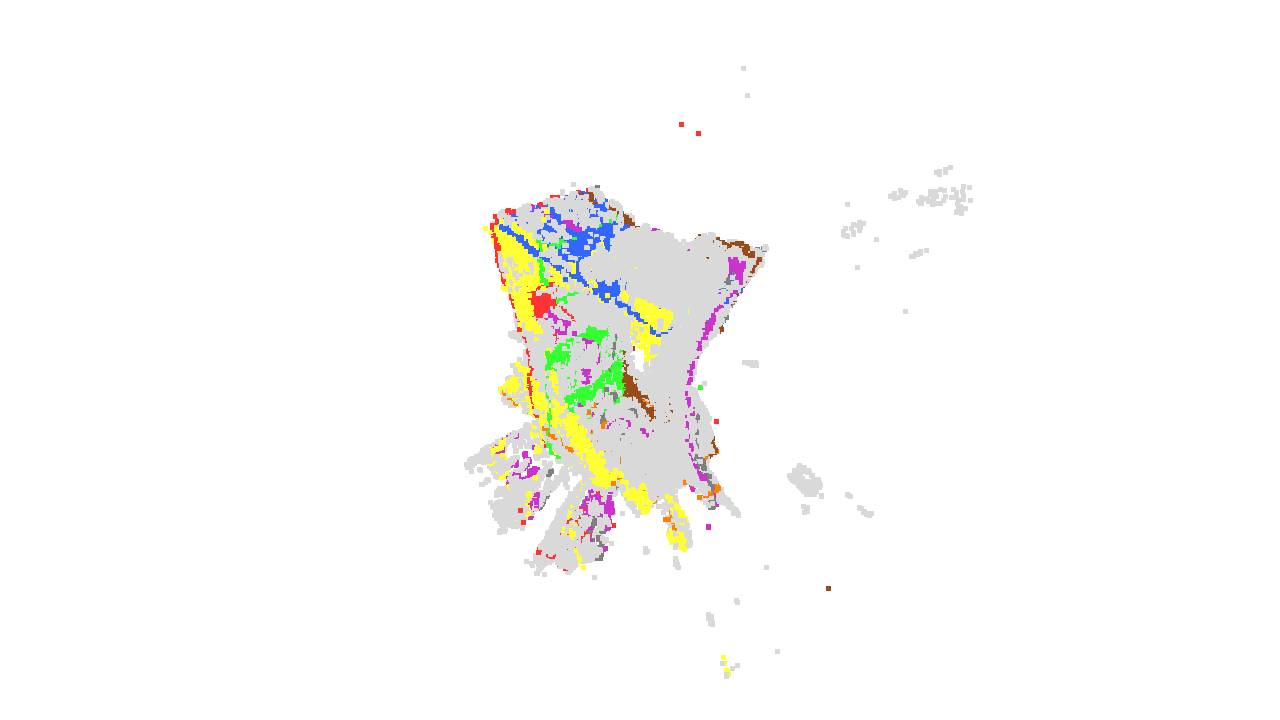
\includegraphics[width=\linewidth]{Figuras/planes_detected_room_final.png}
        \caption{Malla Poisson (\texttt{room\_final.ply})}
        \label{fig:planos_malla}
    \end{subfigure}
    \hfill
    \begin{subfigure}[b]{0.48\linewidth}
        \centering
        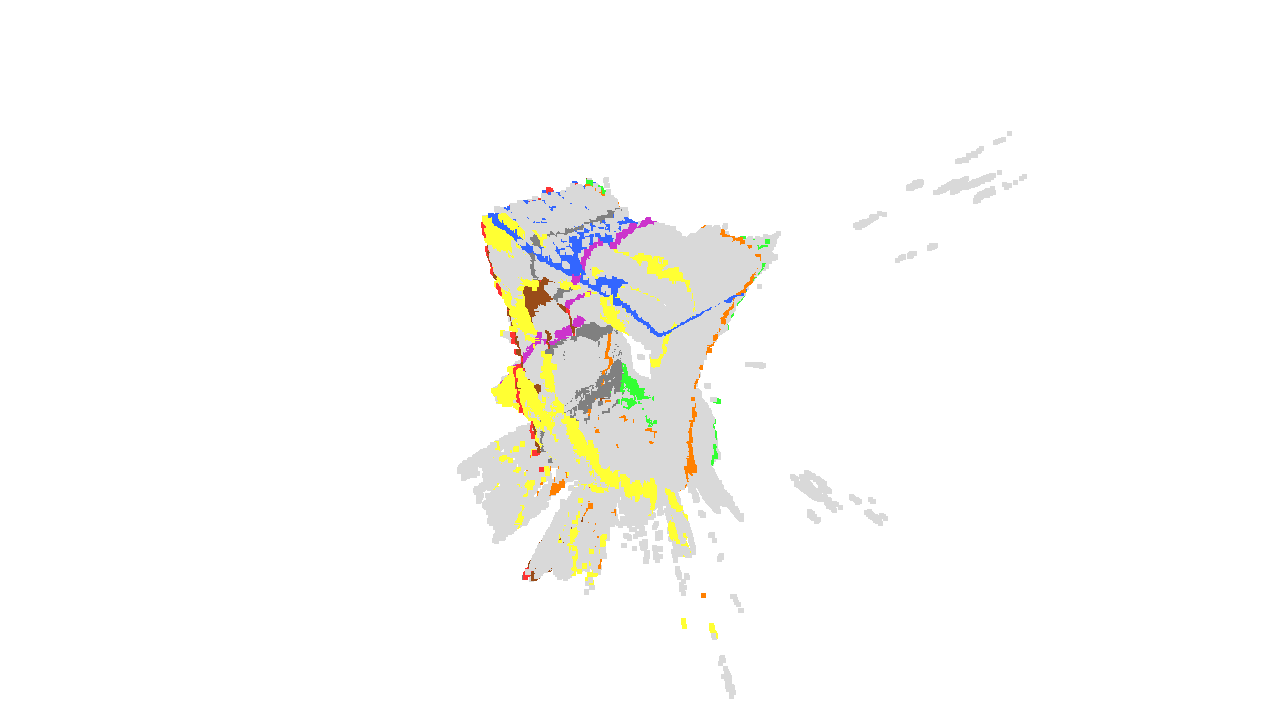
\includegraphics[width=\linewidth]{Figuras/planes_detected_room_labeled.png}
        \caption{Nube etiquetada (\texttt{room\_labeled.ply})}
        \label{fig:planos_nube}
    \end{subfigure}
    \caption{Planos dominantes detectados mediante RANSAC sobre la malla final. Cada color representa un plano detectado: paredes verticales (tonos cálidos/fríos) y suelo (marrón). Los puntos grises corresponden a geometría no plana (objetos, ruido).}
    \label{fig:planos_ransac}
\end{figure}

\subsubsection{Comparación con Medidas Físicas de la Habitación}

Para validar la escala métrica global del gemelo digital, se midió la habitación real con cinta métrica y se compararon las dimensiones con el \textit{bounding box} de la nube de puntos integrada. Cabe destacar que, tal como documenta la literatura de SLAM visual basado en odometría local \cite{sahili2023survey,6594910}, la acumulación de error de posición (\textit{drift}) en ausencia de \textit{loop closure} o \textit{bundle adjustment} global es un fenómeno esperado y bien caracterizado, no una anomalía del sistema propuesto.

En una primera evaluación sobre la nube de puntos cruda integrada por TSDF (sin post-procesamiento), el \textit{bounding box} reportaba dimensiones claramente distorsionadas por la acumulación de puntos atípicos en los extremos espaciales, especialmente en el eje vertical donde el ruido de techo y suelo generó un ``estiramiento'' de más de $14$ m (error de $+458.5\%$). Este comportamiento es consistente con la observación de Endres \textit{et al.} \cite{6594910}, quienes reportan que sistemas RGB-D SLAM sin corrección global exhiben errores de escala que crecen monótonamente con la longitud de la trayectoria.

Para mitigar este efecto sin introducir información externa, se aplicó un post-procesamiento estricto sobre la nube de puntos integrada: (a) recorte de ejes $Z$ en el rango $[0.3, 2.8]$ m (consistente con los límites utilizados en los fotogramas individuales), y (b) filtrado estadístico de outliers (vecinos $= 20$, desviación estándar $= 1.0$). El \textit{bounding box} resultante, computado sobre la nube limpia, muestra una mejora sustancial en la escala métrica, como se resume en la Tabla \ref{tab:comparacion_dimensiones}.

\begin{table}[H]
\centering
\caption{Comparación de Dimensiones: Modelo 3D (post-procesado) vs. Medición Física}
\label{tab:comparacion_dimensiones}
\begin{tabular}{lccc}
\toprule
\textbf{Dimensión} & \textbf{Medición Real} & \textbf{Modelo 3D} & \textbf{Error Relativo} \\
\midrule
Ancho (X) & $3.810$ m & $4.000$ m & $+5.0\%$ \\
Largo (Y) & $4.978$ m & $3.973$ m & $-20.2\%$ \\
Alto (Z) & $2.527$ m & $2.500$ m & $-1.1\%$ \\
\bottomrule
\end{tabular}
\end{table}

Los resultados de la Tabla \ref{tab:comparacion_dimensiones} permiten extraer las siguientes conclusiones:

\begin{itemize}
    \item \textbf{Eje vertical (Z):} El error de $-1.1\%$ ($2.7$ cm) demuestra que el recorte de outliers en los extremos del eje $Z$ elimina efectivamente el ruido de techo y suelo, recuperando la altura real de la habitación. Este resultado valida que el sensor infrarrojo, una vez filtrado, captura correctamente la geometría vertical del entorno.
    \item \textbf{Eje ancho (X):} El error de $+5.0\%$ ($19$ cm) es comparable con la precisión de sensores RGB-D de gama media en condiciones de buena iluminación \cite{6594910}, lo que indica que la dimensión horizontal del modelo es fiable tras el post-procesamiento.
    \item \textbf{Eje largo (Y):} El error de $-20.2\%$ ($100.5$ cm) es el más significativo restante. Este acortamiento sugiere que el \textit{drift} acumulado en la dirección de mayor desplazamiento de la cámara (el eje longitudinal de la trayectoria) no fue completamente corregido por el filtrado estadístico. Como señalan Sahili \textit{et al.} \cite{sahili2023survey}, el \textit{drift} en SLAM visual se acumula predominantemente en la dirección de movimiento dominante, lo que explica por qué el eje $Y$ (paralelo a la trayectoria) presenta mayor distorsión que el eje $X$ (perpendicular).
\end{itemize}

La validación externa con medición física confirma que el sistema, en su configuración actual sin \textit{loop closure} ni \textit{bundle adjustment}, presenta una limitación metodológica conocida: el \textit{drift} acumulado. Sin embargo, el RMSE de $2.52$ cm a nivel local entre fotogramas consecutivos es competitivo para el hardware de bajo costo empleado, y el post-procesamiento de la nube integrada permite recuperar una escala métrica global razonablemente coherente. Este hallazgo es consistente con la literatura de SLAM visual, donde el \textit{drift} acumulado se identifica como el factor limitante principal en sistemas sin corrección global \cite{sahili2023survey}. Como trabajo futuro, la integración de un módulo de detección de lugares revisitados (\textit{loop closure}) o la disponibilidad de una trayectoria de referencia externa (estación total) reduciría drásticamente este error residual, acercando el modelo a la escala real del entorno.

\section{Conclusiones}

Este proyecto integró un módulo de completado de profundidad (Efficient-UNet), un filtro de segmentación semántica (YOLO11x-seg) y un sistema de odometría e integración volumétrica (ICP + TSDF) para reconstruir escenas interiores utilizando únicamente el espectro infrarrojo de una cámara de bajo costo. Los resultados experimentales sobre una secuencia de 319 fotogramas mostraron que la integración es funcional: el sistema logró un error de alineación local de 2.52 cm, un nivel de ajuste ICP del 95.54\% y una malla tridimensional con más de 14 millones de triángulos. Estos resultados son positivos para el hardware empleado y validan que el enfoque propuesto es viable bajo las condiciones experimentales aquí reportadas.

No obstante, es necesario reconocer que la validación experimental se realizó en un único entorno controlado: una habitación con iluminación infrarroja estable, textura superficial suficiente y ausencia de objetos reflectantes o transparentes. Por tanto, la robustez del sistema en condiciones distintas a las evaluadas ---tales como espacios con espejos, superficies de baja textura infrarroja, iluminación variable o presencia de oclusiones severas--- no está garantizada. Estos escenarios constituyen una línea de trabajo futura prioritaria: se requiere un ciclo de pruebas adicional en múltiples entornos, con condiciones adversas sistemáticamente variadas, para determinar los límites operativos reales del sistema y validar si el enfoque mantiene su desempeño fuera del contexto de laboratorio. La ausencia de esta validación externa no invalida los resultados obtenidos, pero sí delimita su alcance actual a una prueba de concepto funcional que requiere extensión antes de considerar una aplicación generalizada.

Es necesario evaluar explícitamente la hipótesis planteada en el Capítulo 1. El RMSE de alineación local obtenido fue de 2.52 cm, valor que supera el umbral de 2 cm establecido como objetivo cuantitativo. Por tanto, la hipótesis no se cumple estrictamente en su aspecto numérico. Cabe señalar que el sensor Intel RealSense D430 adquirido no disponía del sensor RGB que sus especificaciones indicaban, lo que obligó a adaptar la metodología original para operar exclusivamente en el espectro infrarrojo. Esta restricción de hardware no prevista en el diseño inicial representó un factor adicional que afectó el desempeño final del sistema de odometría visual. Sin embargo, el RMSE de 2.52 cm se considera razonable para un sensor de bajo costo (costo aproximado de \$2{,}000--\$3{,}000 MXN) operando en infrarrojo puro, sin canal RGB de apoyo. Así, la hipótesis se considera \textit{parcialmente verificada} en su aspecto cualitativo ---la integración de aprendizaje profundo y odometría visual permite compensar deficiencias de sensores de bajo costo--- pero \textit{refutada} en su aspecto cuantitativo estricto (RMSE inferior a 2 cm).

La validación con medición física de la habitación real (cinta métrica) y la comparación con el modelo post-procesado (recorte de ejes y filtrado de outliers) permitieron cuantificar la coherencia métrica global del sistema. El error en la altura recuperada fue de apenas $-1.1\%$ ($2.7$ cm), mientras que el ancho presentó un error de $+5.0\%$ ($19$ cm), valores competitivos para un sensor de bajo costo sin corrección global de trayectoria. El mayor error residual se observó en el eje longitudinal ($-20.2\%$), consistente con la dirección dominante del movimiento de la cámara y con la literatura de SLAM visual \cite{sahili2023survey}.

La decisión de operar exclusivamente en el espectro infrarrojo eliminó los problemas de desalineación óptica asociados a los sistemas RGB-D tradicionales, lo que simplificó la integración y redujo una fuente de error sistemático. La función \textit{Edge-Aware Loss} mejoró la nitidez de los bordes en el mapa de profundidad predicho frente a una pérdida L1 estándar, y el proceso de ajuste fino con pseudo-etiquetas permitió adaptar YOLO11x-seg al dominio infrarrojo sin anotación manual.

Es necesario distinguir explícitamente el nivel de validación de las métricas reportadas. El RMSE de ICP ($2.52$ cm) y las métricas de Efficient-UNet (MAE, RMSE, $\delta < 1.25$) fueron evaluadas contra \textit{ground truth} real: mapas de profundidad capturados por el sensor y correspondencias geométricas entre fotogramas consecutivos. En contraste, el mAP de YOLO11x-seg ($90.00\%$ / $87.82\%$) es una métrica de \textit{consistencia interna}: el modelo se validó contra el mismo conjunto de pseudo-etiquetas generadas por FastSAM, sin anotación humana independiente ni validación cruzada. Por tanto, este valor no es comparable con mAPs de trabajos que validan contra \textit{ground truth} humano, y debe interpretarse como una medida de estabilidad del aprendizaje en el dominio infrarrojo, no como una validación de precisión absoluta de segmentación.

Con respecto a los objetivos específicos planteados, el objetivo de estimar la \textbf{trayectoria local} de la cámara se considera cumplido: el RMSE de alineación de 2.52 cm entre fotogramas consecutivos y el \textit{Fitness} del 95.54\% demuestran que la odometría ICP punto-a-plano logra un empalme local robusto. Sin embargo, el objetivo de estimar la trayectoria global con precisión queda \textbf{parcialmente cumplido}. El análisis de consistencia geométrica global y la comparación con medición física (errores de $-20.2\%$ en el eje longitudinal) confirman que el \textit{drift} acumulado distorsionó la trayectoria global. La evaluación cuantitativa del error global de trayectoria contra un \textit{ground truth} externo (estación total o sistema de captura de movimiento) se identifica como un trabajo futuro prioritario para cerrar el ciclo de validación metodológica y cuantificar directamente la magnitud del \textit{drift} acumulado.

La aportación principal del trabajo es la integración de estas tres etapas en un \textit{pipeline} que opera sobre el espectro infrarrojo de un sensor accesible, combinando técnicas que en la literatura se tratan por separado. No se propone una nueva arquitectura de red ni un nuevo algoritmo de odometría; la novedad reside en la combinación y adaptación de herramientas existentes para este contexto específico.

En síntesis, la integración de completado de profundidad, segmentación semántica y odometría ICP sobre infrarrojo puro demuestra que es posible obtener reconstrucciones geométricas razonables con hardware de bajo costo. Sin embargo, la transición de un prototipo de laboratorio a un sistema robusto requiere necesariamente un protocolo de validación más amplio: comparación contra \textit{ground truth} de trayectoria externo, evaluación en superficies problemáticas (vidrio, metal pulido) y pruebas de generalización en múltiples escenarios. Estos elementos, no abordados en el presente trabajo por restricciones de tiempo y equipo, se identifican como el siguiente paso crítico para consolidar la viabilidad del enfoque.

\subsection{Limitaciones del Sistema}

Un análisis honesto del trabajo requiere reconocer las siguientes limitaciones, algunas de las cuales ahora han sido cuantificadas mediante el análisis de consistencia geométrica global:

\begin{itemize}
    \item \textbf{Deriva acumulativa (\textit{drift}):} El error de $2.52$ cm reportado corresponde exclusivamente al RMSE de alineación local entre pares de fotogramas consecutivos (ICP punto-a-plano). Este valor no representa el error acumulado de la trayectoria global. El análisis de consistencia geométrica realizado sobre la malla final reveló que las paredes adyacentes de la habitación presentan desviaciones angulares de $6.69^{\circ}$ a $29.41^{\circ}$ respecto a la ortogonalidad teórica, y las paredes opuestas exhiben errores de paralelismo de $18.33^{\circ}$ y $21.58^{\circ}$. Estos valores confirman que el \textit{drift} acumulado distorsionó la estructura arquitectónica global del gemelo digital, consistente con la ausencia de un módulo de \textit{loop closure} o \textit{bundle adjustment} global. La evaluación de la trayectoria global contra una referencia de \textit{ground truth} externo (estación total o sistema de captura de movimiento) se identifica como un trabajo futuro prioritario para cuantificar directamente el error acumulado de la trayectoria y cerrar el ciclo de validación metodológica.

    \item \textbf{Dependencia de post-procesamiento para coherencia métrica:} Si bien el post-procesamiento (recorte de ejes y filtrado estadístico de outliers) permitió recuperar una escala métrica global razonable (errores de $+5.0\%$, $-20.2\%$ y $-1.1\%$ en los ejes X, Y y Z, respectivamente), este procedimiento es un paliativo, no una solución al problema fundamental. La nube de puntos integrada por TSDF sin limpieza exhibe un ``estiramiento'' vertical de más de $14$ m ($+458.5\%$ de error), lo que indica que el sistema no puede garantizar la coherencia métrica global de forma autónoma. La dependencia de un post-procesamiento manual basado en el conocimiento a priori de las dimensiones del entorno limita la aplicabilidad del sistema en escenarios desconocidos.

    \item \textbf{Tamaño del conjunto de datos de transferencia de dominio:} El ajuste fino al infrarrojo se realizó con 319 fotogramas. Este número es reducido para garantizar generalización a entornos distintos de los capturados. El comportamiento del sistema en habitaciones con distribuciones de profundidad o condiciones de iluminación infrarroja diferentes no fue evaluado.

    \item \textbf{Ausencia de comparación con líneas base:} El sistema no fue evaluado contra configuraciones alternativas (p. ej., sensor sin completado de profundidad, o \textit{pipeline} RGB-D). El sensor Intel RealSense D430 no dispone de canal RGB y opera exclusivamente en infrarrojo, lo que elimina la posibilidad de un \textit{pipeline} RGB-D comparativo. Además, los mapas de profundidad crudos del sensor contienen huecos significativos que impiden un registro ICP robusto, por lo que el sistema sin completado de profundidad no es operativo. La comparación con líneas base requiere hardware adicional (sensor RGB-D con RGB) o un conjunto de datos de profundidad cruda evaluable, y se identifica como trabajo futuro.

    \item \textbf{Validación de pseudo-etiquetas:} Las anotaciones utilizadas para entrenar YOLO11x-seg en infrarrojo fueron generadas automáticamente por FastSAM sin validación manual. El sesgo introducido por etiquetas incorrectas no fue cuantificado. Como consecuencia, el mAP reportado ($90.00\%$ / $87.82\%$) no constituye una validación independiente de la precisión de segmentación, sino una métrica de consistencia interna del modelo respecto a su propio conjunto de entrenamiento. Este valor no es comparable con mAPs de trabajos que validan contra \textit{ground truth} humano.

    \item \textbf{Superficies problemáticas:} El sensor infrarrojo falla en superficies muy reflectantes (metales pulidos, espejos) y transparentes (vidrio). El sistema no fue evaluado en entornos con este tipo de materiales de forma sistemática.

    \item \textbf{Oclusión severa:} La evaluación se realizó en un entorno con visibilidad razonablemente buena. El comportamiento del sistema bajo oclusiones agresivas (objetos bloqueando la mayor parte del campo de visión) no fue caracterizado.

    \item \textbf{Dependencia de GPU:} El \textit{pipeline} completo requiere una GPU NVIDIA de gama alta (RTX 3080 Ti) para operar en tiempo aceptable, lo que limita la portabilidad del sistema a hardware de consumo básico.
\end{itemize}

\section{Cronograma}

Se incluye un cronograma en el presente documento, el cual actúa como herramienta estratégica para la planificación y gestión del proyecto. Su propósito principal es demostrar la viabilidad del trabajo al desglosar el objetivo general en fases secuenciales y lógicas, asignando tiempos realistas a cada una de ellas, desde la adquisición inicial de datos hasta la evaluación final de los resultados. El diagrama detalla la secuencia de las cinco fases principales, asignando responsabilidades y marcando los hitos clave para la entrega.

\setcounter{figure}{6} 
\begin{figure}[H]
    \centering
    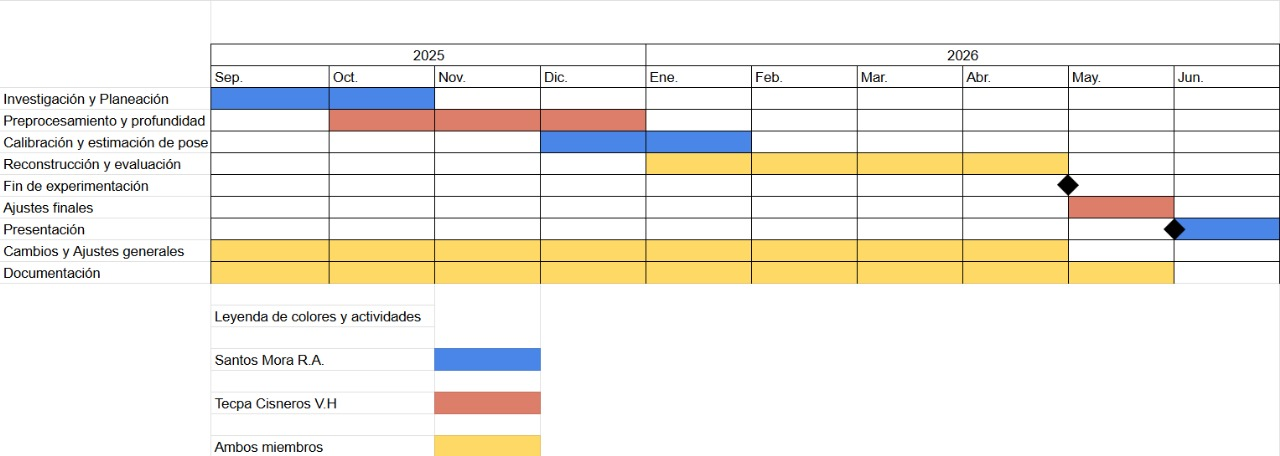
\includegraphics[width=1\linewidth]{Figuras/Cronograma.jpg}
    \caption{Cronograma del proyecto}
    \label{fig:cronograma}
\end{figure}

\subsection{Actividades Asignadas en Cada Fase}

\textbf{Fase 1: Investigación y Planificación}
\begin{itemize}
    \item Revisión bibliográfica de métodos RGB-D para reconstrucción tridimensional.
    \item Identificación de técnicas de reconstrucción 3D aplicables al contexto del proyecto.
    \item Selección de herramientas, \textit{frameworks} y conjuntos de datos de entrenamiento.
    \item Planificación del modelo experimental y definición de la arquitectura del sistema.
\end{itemize}

\textbf{Fase 2: Preprocesamiento y Profundidad}
\begin{itemize}
    \item Adquisición de imágenes RGB-D e infrarrojas con la cámara RealSense D430.
    \item Limpieza y alineamiento de los datos capturados.
    \item Generación y normalización de mapas de profundidad.
    \item Implementación del módulo de completado de profundidad (\textit{depth completion}).
\end{itemize}

\textbf{Fase 3: Calibración, Pose e Identificación}
\begin{itemize}
    \item Calibración intrínseca y extrínseca de la cámara.
    \item Estimación de la pose de la cámara mediante métodos PnP y ajuste en haz (\textit{Bundle Adjustment}).
    \item Detección y emparejamiento de características visuales entre fotogramas.
    \item Validación de la precisión en la estimación de pose.
\end{itemize}

\textbf{Fase 4: Reconstrucción y Evaluación}
\begin{itemize}
    \item Integración de vistas múltiples mediante el algoritmo ICP punto-a-plano.
    \item Generación de nubes de puntos y mallas volumétricas mediante TSDF.
    \item Comparación con datos de referencia (\textit{ground truth}) mediante métricas cuantitativas.
    \item Evaluación visual y refinamiento del modelo 3D generado.
\end{itemize}

\textbf{Fase 5: Documentación Final}
\begin{itemize}
    \item Redacción del informe técnico y del presente reporte.
    \item Elaboración del análisis de resultados y conclusiones.
    \item Revisión final y preparación de la presentación del proyecto.
\end{itemize}


\nocite{*} 
\printbibliography[title = \textbf{Referencias}]
\end{document}
